%=================================================================
%				preamble
%=================================================================
\documentclass[11pt,letterpaper]{book}

\newcommand{\theauthor}{Thomas Graf}
\newcommand{\lastname}{Graf}
\newcommand{\university}{Stony Brook University}	
\newcommand{\emailaddress}{lin637@thomasgraf.net}
\newcommand{\coursenumber}{Lin637}
\newcommand{\coursename}{Computational Linguistics 2}
\newcommand{\semester}{Spring 2015}
\newcommand{\thetitle}{\coursename\ [\coursenumber, \semester]}
\newcommand{\thekeywords}{graduate level, lecture, computational linguistics, phonology, syntax}
\newcommand{\thedate}{}

\usepackage{mypackages}
\usepackage{mycommands}


%=================================================================
%			title format
%=================================================================
\author{\theauthor}
\title{\thetitle}
\date{\thedate}

%=================================================================
%			content
%=================================================================
% \includeonly{./tex/ConstituencyTests}

\pagestyle{empty}
\begin{document}
\maketitle
\raggedbottom
\pagenumbering{Roman}
\tableofcontents
\clearpage

\setcounter{chapter}{-1}
\chapter{Syllabus}
\label{cha:syllabus}
\setcounter{page}{1}

\fcolorbox{gray!25}{gray!25}{%
    \centering
    \begin{tabular}{ll}
        \textbf{Course:} Computational Linguistics 2&
        \textbf{Name:} Thomas Graf\\
        \textbf{Course\#:} Lin637 &
        \textbf{Email:} \href{mailto:lin637@thomasgraf.net}{lin637@thomasgraf.net}\\
        \textbf{Time:} TR 10:00--11:20am &
        \textbf{Office hours:} tba \\
        \textbf{Location:} Humanities 2047 &
        \textbf{Office:} SBS N249\\
        \textbf{Course Website:} \href{http://lin637.thomasgraf.net} {lin637.thomasgraf.net} &
        \textbf{Personal Website:} \href{http://thomasgraf.net}{thomasgraf.net}
    \end{tabular}
}

\section{Course Outline}

\subsection{Bulletin Description}
An introduction to the theoretical foundation of computational linguistics.
The course emphasizes the importance of algorithms, algebra, logic, and formal language theory in the development of new tools and software applications.
Empirical phenomena in phonology and syntax are sampled from a variety of languages to motivate and illustrate the use of concepts such as strictly local string languages, tree transducers, and semirings.
Students will develop familiarity with the literature and tools of the field.

\subsection{Full Description}

This course serves a specific purpose in our program (see Fig.~\vref{fig:Syllabus_Program}):
it acts as the bridge from introductory courses in linguistics (Syntax 1, Phonology 1, Phonetics) and computational methods (Statistics, Mathematical Methods in Linguistics, Computational Linguistics 1) to advanced courses and seminars in computational\slash mathematical linguistics.
In contrast to the NLP courses offered by the department of computer science, our courses focus on studying the properties of natural language from a computationally informed perspective.
The question is not how computers can solve linguistic tasks, but how language can be conceptualized as a computational problem.
This emphasis is also reflected in the selection of topics for this course.

\begin{itemize}
    \item \textbf{What this course is not about}
        \begin{itemize}
            \item Computer-assisted research methods in linguistics
            \item Programming
            \item Software development for natural language tasks
        \end{itemize}
    \item \textbf{What is not covered but benefits from what is covered}
        \begin{itemize}
            \item Speech recognition
            \item OCR
            \item Text generation
            \item Parsing
            \item Semantic analysis
            \item Machine translation
        \end{itemize}
    \item \textbf{List of topics}
        \begin{itemize}
            \item \emph{Phonology and Morphology}
                \begin{itemize}
                    \item The role of formalization
                    \item String languages
                    \item Subregular hierarchy
                    \item Regular languages
                    \item Generative capacity of phonology
                    \item String transductions
                    \item 2-level morphology
                    \item Equivalence of SPE and OT
                \end{itemize}
            \item \emph{Syntax}
                \begin{itemize}
                    \item Tree languages
                    \item Syntax is more complex than phonology
                    \item Mildly context-sensitive formalisms (TAG, MGs)
                    \item Tree transductions
                    \item Regular representations of MCS formalisms
                    \item Reinterpreting the T-model
                \end{itemize}
        \end{itemize}
\end{itemize}

A rough outline of the course progression is given in Tab.~\vref{tab:Syllabus_CourseOutline}.
Many of the topics we cover draw from very specialized areas of formal language theory that even most mathematicians and computer scientists do not know about, e.g.\ the correspondence between finite-state machines and monadic second-order logic, or the logical characterization of tree transductions.
So this course might be of value to you even if you do not particularly care about natural language.
Make no mistake, though, we'll talk a lot about language and linguistics --- this is not a math class.

\begin{table}
    \centering
    \begin{tabular}{rp{5.5cm}p{5.5cm}}
        \toprule
        \emph{Wk} & \emph{Formal} & \emph{Linguistics} \\
        \toprule
        1         & What is computation? & Marr's Three Levels\\
        2         & Formalizing phonology & Why formalize?\\
        3         & Strictly local languages & Local dependencies\\
        4         & Subregular hierarchy & How powerful is phonology?\\
        5         & Regular languages & Abstractness\\
        6         & String transductions & SPE-OT equivalence\\
        7         & Two-level morphology & Null morphemes\\
        \midrule
        8         & (Spring Break) & \\
        \midrule
        9         &  Weak Generative Capacity & $\text{Phonology} < \text{Syntax}$\\
        10        &  Tree languages & Headedness, feature percolation\\
        11        &  Local tree languages & GPSG\\
        12        &  Recognizable tree languages & GB\\
        13        &  TAG and MGs & Minimalist syntax\\
        14        &  Tree transductions & Reinterpreting the T-model\\
        15        &  Unification via first-order logic & Strictly Derivational Minimalism\\
        \bottomrule
    \end{tabular}
\caption{Tentative course outline}
\label{tab:Syllabus_CourseOutline}
\end{table}

\begin{figure}
    \rotatebox{0}{
        \footnotesize
        \begin{tikzpicture}[
    every node/.style = { draw, thick },
    every path/.style = { ->, thick },
    sug/.style = { dashed },
    req/.style = { },
    ]
    \node (CL2) at (0,0) [align=center] {Computational Linguistics 2\\ (Lin 637)};

    % Prereqs
    \node (Phon) [above=of CL2, xshift=-8em, align=center] {Phonology 1 (Lin 522)\\
                                                                \emph{or}\\
                                                            Phonetics (Lin 523)
                                                        };
    \node (Syntax) [left=of Phon, align=center] {Syntax 1\\ (Lin 521)};
    \node (Math)   [above=of CL2, xshift=8em, align=center] {Statistics (Lin 538)\\
                                                                \emph{or}\\
                                                            Mathematical Methods (Lin 539)
                                                        };
    \node (CL1) [right=of Math, align=center] {CompLing 1\\ (Lin 537)};

    % CS branch
    \node (NLP) [below right=of CL2, xshift= 8em, align=center] {Introduction to NLP\\ (CSE 628)};
    \node (Machine) [below=of NLP, xshift=-8em, align=center]  {Machine Learning\\ (CSE 512)};
    \node (Speech)  [below=of NLP, xshift= 8em, align=center] {Speech Processing\\ (CSE 542)};

    % Linguistics branch
    \node (CompSem) [below=of CL2, xshift=-16em, align=center] {Computational Semantics\\ (Lin 626)};
    \node (CompPhon) [below=of CompSem, align=center] {Computational Phonology\\ (Lin 627)};
    \node (CompSyn) [below=of CompPhon, align=center] {Computational Syntax\\ (Lin 628)};

    \node (Learn) [right=of CompSem, xshift=4em, align=center]  {Learnability\\ (Lin 629)};
    \node (Parse) [right=of CompPhon, xshift=4em, align=center] {Parsing and Processing\\ (Lin 630)};

    % Branches
    \draw[sug] (Syntax) |- (CL2);
    \draw[sug] (Phon) to (CL2);
    \draw[sug] (Math) to (CL2);
    \draw[req] (CL1) |- (CL2);
    \draw[req] (CL1.south -| NLP.north) -- (NLP);
    \draw[sug] (NLP) -| (Machine);
    \draw[sug] (NLP) -| (Speech);
    \draw[sug] (Learn |- CL2.south) -- (Learn); 
    \draw[sug, transform canvas={xshift=2em}] (Parse |- CL2.south) -- (Parse);
    \draw[sug] ($(CL2.south)-(6em,0)$) |- (CompSem);
    \draw[sug] ($(CL2.south)-(5em,0)$) |- (CompPhon);
    \draw[sug] ($(CL2.south)-(4em,0)$) |- (CompSyn);
\end{tikzpicture}

    }
\caption{Computational Linguistics 2 in the curriculum (dashed lines indicate recommendations rather than prerequisites)}
\label{fig:Syllabus_Program}
\end{figure}    

\subsection{Prerequisites}

The only official prerequisite is Computational Linguistics 1 (Lin 537) or comparable programming skills in Python.
Python will be used to illustrate some formal concepts, and some of the homeworks will require you to implement an algorithm or procedure in Python.
Prior experience with git, markdown, and \LaTeX\ is useful for the homeworks but not required.

It is also helpful to have some basic familiarity with linguistics (phonemes, phrase structure rules, syntactic trees) and mathematics (sets, functions, relations, and first-order logic as covered in Semantics 1, for instance).
You can take an online survey to identify weaknesses, and several introductory readings on these topics are available on the course website.

\medskip
\noindent
\hspace{-.75em}
\begin{tabular}{ll}
    \textbf{Survey URL:} & 
    \href{https://testmoz.com/432409}{https://testmoz.com/432409}\\
    \textbf{Password (if required):} &
    CompLing2
\end{tabular}

\section{Teaching Goals}
\begin{itemize}
    \item \textbf{Practical Skills}
        \begin{itemize}
            \item conceptualize a problem in mathematical terms
            \item optimize your programs through the use of adequate algorithms and data structures (dynamic programming techniques, hash tables, etc.)
            \item a more abstract and theoretically informed perspective on current tools and techniques in NLP
            \item an understanding for how linguistic insights can be invoked to simplify NLP tasks
        \end{itemize}
    \item \textbf{Research Skills}
        \begin{itemize}
            \item assess linguistic phenomena from a computational perspective
            \item evaluate linguists' claims about computational efficiency
            \item basic overview of current research in theoretical computational linguistics
            \item use computational concepts to identify new empirical generalizations
            \item bring linguistic data to bear on computational claims
            \item mathematically informed understanding of linguistic theories
        \end{itemize}
\end{itemize}


\section{Grading}
\begin{itemize}
    \item \textbf{Homework}
        \begin{itemize}
            \item weekly exercises, programming assignments, or critical evaluations of assigned readings
            \item Homework submission and grading is done via github.
            \item No late hand-ins!
            \item Collaboration on homework problems is encouraged as long as you write up the solutions by yourself, using your own words, examples, notation, and code.
        \end{itemize}
        %
    \item \textbf{Readings}
        \begin{itemize}
            \item about two readings per week
            \item you have to collaboratively write a summary for each reading in the course wiki
        \end{itemize}
        %
    \item \textbf{Survey Squibs}
        \begin{itemize}
            \item By the end of the course, the wiki should contain survey articles on a number of topics not covered in this course (or not covered at the same depth).
            \item You have to pick a topic and write the corresponding survey article.
            \item These articles should be succinct and simple enough that they are comprehensible to a researcher with little exposure to computational linguistics, yet at the same time include enough technical detail that the claims can be verified by somebody with the appropriate background.
                (Why this weird requirement?
                Because that's the recipe for writing a computational paper that can be published in a linguistics journal!)
        \end{itemize}
        %
    \item \textbf{Workload per Credits}
        \begin{itemize}
            \item \emph{3 credits}: homework, readings, squib
            \item \emph{2 credits}: homework, readings
            \item \emph{1 credit}: readings
            \item \emph{0 credits}: none, but I highly recommend that you at least read the assigned papers as they will be important for following the lectures
        \end{itemize}
\end{itemize}


\section{Online Component}

This class uses some online tools to facilitate homework collaboration and submission, student discussions, and dynamic lecture evaluation.

\begin{itemize}
    \item \textbf{Homework submission}\\
        \emph{How it works:}
        Homeworks will distributed via a github repository. 
        You can fork this repo and upload your own code, or checkout other students' forks to see how they dealt with the problem.
        In order to submit a homework you upload your solution to your fork and issue a pull request.
        After the due date, I'll upload my solution to the repository.

        \emph{Why we do it:}
        This setup mimics the modern workflow in collaborative development projects.
        Git is one of the best-known version control systems, and github is the biggest online service for hosting git repositories.
        Familiarity with version control systems is an essential job requirement for computational linguists, and it is also very helpful for academic work.
        See this discussion on Stackflow for some ideas how git can be used in conjunction with Latex:
        \href{http://stackoverflow.com/questions/6188780/git-latex-workflow}{http://stackoverflow.com/questions/6188780/git-latex-workflow}

        \emph{What you'll need:}
        A github account (the free tier is enough) and a way of uploading your code to a github repository. Linux users can install git via the command line, whereas Windows and Mac users should download and install the github app, which comes with a nice GUI.

    \item \textbf{Homework Feedback and Discussion}\\
        \emph{How it works:}
        Every github repository comes with an issue (= ticket) tracker.
        If you have a question or wish to discuss a topic, you can open a ticket on the main repository (note: tickets support markdown).
        I may also use tickets to leave comments on your homeworks.

        \emph{Why we do it:}
        Once again this is an essential part of modern software development.
        And it is also a lot more convenient than anything Blackboard has to offer.

        \emph{What you'll need:}
        Not much beyond the ability to navigate the github repos.

    \item \textbf{Reading summaries}\\
        \emph{How it works:}
        Every week I create an empty page on the course wiki for each assigned reading.
        Your job is to expand these articles into useful summaries.
        The default syntax for the wiki entries is markdown, a very simple \emph{lingua franca} for writing plain text documents that can easily be converted into a variety of file formats (doc, pdf, html, and so on).

        \emph{Why we do it:}
        Wikis are frequently used for software documentation nowadays, so you have to know how to work with one.
        You will also get to see the advantages of markdown, in particular for short documents that do not need a lot of fancy typesetting (this can even include your own website!).
        Hopefully this will move you away from formats like doc, which
        %
        \begin{itemize*}
            \item are proprietary, and
            \item lack backwards compatibility, and
            \item are tedious to index and search, and
            \item fail to separate the content of a document from its presentation, thereby distracting you with unnecessary details.
        \end{itemize*}
        %
        Also, learning markdown takes a lot less time than relearning the MS Office user interface with each new version.
        If you find that markdown is too simple for your own purposes, you can also switch to a more expressive superset like \href{http://johnmacfarlane.net/pandoc/}{pandoc}.

        \emph{What you'll need:}
        Nothing except the ability to read (and ideally write in) markdown.
        The github editor makes this fairly easy with its built-in help, formatting buttons and dynamic preview.
        You can also checkout this interactive markdown tutorial, which should take you about 15 minutes (yes, markdown is that easy!):
        \href{http://markdowntutorial.com/}{http://markdowntutorial.com/}

    \item \textbf{Class announcements}\\
        \emph{How it works:}
        Normal announcements (readings, due dates) are put on the course website, time-critical ones (i.e.\ class cancellations) are emailed out via Blackboard.
        
        \emph{What you'll need:}
        If you're not officially enrolled in the course, send me a message so I can add you to Blackboard.

    \item \textbf{Handouts}\\
        \emph{How it works:}
        Handouts are made available online Monday and Wednesday before 3pm.
        You can look at them on your laptop\slash tablet or make a hardcopy before class.
        I will not bring handouts to class unless I could not upload them on time the day before.

        \emph{Why we do it:}
        Mostly because I just don't like paper.
        Also keep in mind that you can fork the lecture notes repository and include your notes directly in the Latex source files.
        Then you can compile a version of the lecture notes with your own notes already included.
\end{itemize}


\section{Policies}

\subsection{Contacting me}
\begin{itemize}
    \item Emails should be sent to \href{mailto://lin637@thomasgraf.net}{lin637@thomasgraf.net} to make sure they go to my high priority inbox.
        Disregarding this policy means late replies and is a sure-fire way to get on my bad side.
    \item Reply time < 24h in simple cases, possibly more if meddling with bureaucracy is involved.
    \item If you want to come to my office hours and anticipate a longer meeting, please email me so that we can set apart enough time and avoid collisions with other students.
\end{itemize}

\input{./tex/blabla.tex}


\pagenumbering{arabic}

\chapter{Computation and Formalization}
\label{cha:Formal}

Without a doubt the most unfortunate fact about computational linguistics is that its name is \emph{computational linguistics}.
The term inherits a dichotomy that is hard to tease apart for the uninitiated: the distinction between computers and computing.
While computers are the most common tool for carrying out computations nowadays, they are not what computing is about.
Computation, in its barest form, is the principled manipulation of information.
When a computer verifies $1 + 1 = 2$, this act of computation is instantiated via a series of electrical impulses that affect some of the millions of transistors that make up its hardware.
The same computation will look very different when executed by a human brain, with neurons firing in a specific cascade that gives rise to a three-dimensional activation pattern.
Or maybe we are just dealing with a few beads being moved around in an abacus.
Despite these differences in biological substrates, structural changes, and sheer computing power, all three are equally valid examples of computation.
In fact, the notion of computation is so fundamental a concept that even the universe itself can be viewed as one giant computation --- computers, in contrast, are just a handy gadget for carrying out computations.

\emph{Computational linguistics} is an unfortunate name because it does not clearly disambiguate these two terms: 
\Note{At least it is better than the German term \emph{Computerlinguistik}, which can only have the first meaning when interpreted compositionally.}
are we talking about language and computers, or language and computation?
For the purposes of this course, computational linguistics will always refer to ``language and computation'', while ``language and computers'' will be subsumed under the term \emph{natural language processing} (NLP).
NLP is about solving language-related tasks with computers, e.g.\ speech synthesis, machine translation, or even the basic search function in your text editor.
Computational linguistics is about studying language as an instance of computation.
And that will be our topic for the next 15 weeks.

More precisely, this course is concerned with the computational aspects of natural language and how we can analyze them from a formal perspective.
While it may seem innocuous, this statement is actually very ambiguous and contentious.
What exactly do we mean by \emph{computational aspects}, why should those be interesting questions to ask, and what is the supposed advantage of this \emph{formal perspective} over the proposals made by theoretical linguists?

\section{Computational Linguistics: Why Should Anybody Care?}

\subsection{Practical Arguments}

It seems fairly easy to make a case for the importance of studying computational aspects of language (putting aside for now what exactly we mean by that). 
Usually the first argument to be presented is that a world in which computers can successfully handle all kinds of language-related tasks is preferable to one where they cannot, and consequently it is imperative that we do whatever we can to get computers to this level of aptitude.
And just like some understanding of physics had to be in place before engineers could bless mankind with the radio or the combustion engine, we cannot have successful NLP applications without a minimum understanding of language and the computational challenges it poses.
Computational linguistics thus is a prerequisite for NLP\@.

This argument is too simplistic, though.
One of the most shocking things about the applied sciences and engineering is how little genuine understanding one needs to construct a useful tool.
To give but one example: relativity theory is not an integral part of calculating artillery ballistics.
In many areas of life the allowed margin of error is large enough that shortcuts, hacks, and brute force methods will get the job done.
For practical purposes it is also perfectly fine to make stipulations that fly in the face of scientific consensus but improve the final results.
In the words of Noam Chomsky \citep[147]{Chomsky90}:
%
\begin{quote}
    Throughout history, those who built bridges or designed airplanes often had to make explicit assumptions that went beyond the understanding of the basic sciences.
\end{quote}
%
Similar things can be observed in NLP, where very shallow methods often yield surprisingly useful results.
A word cloud, for instance, requires only the most basic statistics but can summarize texts in a very effective manner.
Things might change in the future as users demand more and more accurate tools for increasingly difficult tasks, but at this stage there is still a large gap between ``language as a computational problem'' and ``computers solving natural language tasks''.

A more refined version of the practical applicability argument points out that while a theoretically informed perspective may not be of any practical use for now, it can lay the foundation for entirely new fields, tools, and businesses in the future.
The poster child for this is of course number theory, which for the longest time was considered a purely theoretical and utterly useless subfield of mathematics but is now the central pillar on which all of modern cryptography rests.
Whether you are encrypting files on your computer or talking to a server through a safe channel, it all builds on number theory.
But we do not have to look at mathematics to see examples of theoretical research giving rise to important new developments, linguistics has several examples of its own.
Formal language theory --- which is an integral part of computer science and indispensable for the design of programming languages and file standards like XML, among other things --- grew out of Chomsky's attempts to develop formal models of natural language syntax.
Chomsky's writings about syntactic transformations also served as an inspiration for William Rounds' \citep{Rounds70} work on tree transducers, which are now used in compiler design and machine translation.
More recently, Aravind Joshi's Tree Adjoining Grammar (TAG) has even been used to model messenger RNA \citep{Uemura.etal99, Matsui.etal05}.
Overall, then, there is ample evidence that theoretical inquiry does benefit practical applications eventually and consequently we may hope that studying the computational aspects of language will benefit not only NLP, but also future areas that we cannot envision at this point.

\subsection{Scientific Arguments}

Utilitarian arguments may convince politicians, taxpayers, and engineers, but they hold no sway in the court of science.
A linguist would shrug at the arguments above on a good day, and publicly denounce us as nimrods on a bad one.
Fortunately, the scientific merit of computational linguistics is a lot more clear-cut: language is intrinsically a computational problem, so it should be studied as such.

\Note{Semantics is noteworthy for being the one subfield of linguistics that is still very strongly aligned with the externalist view of language and does not think of its formalism as the high-level description of a specific part of human cognition.
For a mentalist approach to natural language meaning see \citet{Pietroski14}.
}
Probably the most important development in 20\tsp{th} century linguistics is the \emph{cognitive turn}, the shift from viewing language as an external system of rules and words to its reinterpretation as one of humans' many cognitive abilities.
Language is not an abstract platonic object, it is done by humans, it is an algorithm that runs on the human brain (the \emph{wetware}).
That immediately raises the question how language is computed.

Linguists actually split this up into two subquestions:
%
\begin{description}
    \item[Competence] What is the specification of the computations?
    \item[Performance] How is this specification implemented and used?
\end{description}
%
Competence questions are concerned with the rules of grammar and how they are encoded.
Somewhat sloppily, one could describe competence as ``language modulo resource restrictions like limited working memory and attention span''.
Of course nothing of this sort can be observed in nature --- competence is an artificial abstraction of performance, which is about how the specification behaves when it is run on an actual machine, i.e.\ the human brain.
The distinction between competence and performance also exists in computer science to some extent.
For example, complexity theory studies the difficulty of problems of unbounded size, even though in practice problems are usually bounded, e.g.\ because a computer can only store so much information.
Nonetheless complexity theory has produced results that are also relevant in practice, and competence questions in linguistics have similarly shed some light on performance.

Since competence cannot be directly observed, research into how language is computed usually operates in the realm of performance.
Linguists approach this questions through the lens of neuroscientists and psychologists: how does the wetware behave when carrying out specific linguistic tasks, and can we design a procedure that mimics humans' behavior?
For example, native speakers of English usually have no problem understanding English sentences, it is an incredibly fast and effortless process.
But it does exhibit surprising quirks.
When asked whether the sentence \eqref{ex:Formal_GardenPath} is grammatical, they usually say yes.
%
\begin{exe}
        \ex The player tossed a frisbee smiled.\label{ex:Formal_GardenPath}
\end{exe}
%
However, the sentence is actually grammatical, it has the same structure as the minimally different \eqref{ex:Formal_Non-GardenPath}. 
%
\begin{exe}
    \ex The player thrown a frisbee smiled.\label{ex:Formal_Non-GardenPath}
\end{exe}
%
For some reason the algorithm native speakers of English use has no problem with \eqref{ex:Formal_Non-GardenPath} but is completely thrown off by the exchange of a single word that serves exactly the same grammatical function.
This is almost like a computer that can compute $1 + 2$ but not $2 + 1$.
There is no obvious reason for this behavior, and it doesn't exactly look like good engineering (so much for intelligent design).
Linguists have come up with various elaborate explanations of such phenomena over the years --- some more successful than others ---
but they all share a variety of properties that necessarily limit their scope and thus the questions they can address.

\subsubsection{Neuroscience}

It is certainly interesting to see how the human brain works on the hardware level, but that does not tell us anything about the actual computations --- just like studying a computer's hardware tells us little about what it is computing.
If we hear the hard drive spin up we can make the reasonable assumption that some file is being accessed, but that is about all we can deduce with our own senses.
Inquisitive minds that we are, we may then decide to connect a set of thermal diodes to various points of the hardware in order to detect whether that piece of hardware starts heating up, suggesting an increase of computational activity there.
But that is still very inconclusive, for various reasons.

First of all, a higher load on the graphics chip might indicate that some kind of 3D graphics is being rendered, e.g.\ for a video game, but actually a lot of non-graphical tasks are outsourced from the processor to the graphics chip nowadays.
\Note{Graphics chips are also called Graphics Processing Units (GPUs).
    The usage of GPUs for non-graphical tasks is known as GPGPU: General Purpose Computing on GPUs.}
And even if it were possible to tie each piece of hardware to a specific task,
we still could not determine whether the computer is, say, sorting a list or searching through it, two very different tasks.
More fine-grained distinctions are completely unthinkable, such as whether one of the two search algorithms below is being used, and if so, which one.
%
\begin{center}
    \pythonfile[firstline=5]{./code/list_search/linear_search.py}
\end{center}
\begin{center}
    \pythonfile[firstline=5]{./code/list_search/binary_search.py}
\end{center}
%
The binary search algorithm is a lot more sophisticated than linear search, and it is also much faster on average.
It does have the disadvantage that it only works for sorted lists, so unsorted lists need to be sorted first, and in cases where no sorting order can be defined, the algorithm does not work at all.
So if we had two computers with exactly the same hardware, one using linear search and the other binary search, the latter would show vastly superior performance in general but would fail miserably in specific cases.
The behavior of this computer might even look similar to humans' puzzling problems with certain grammatical sentences.
Yet the behavior cannot be explained in terms of hardware, because we know for a fact that the two machines are exactly the same.

In the case of computers, we have the advantage that we already know how their architecture works because we designed it.
So if that still isn't enough to deduce from the hardware what kind of computations a computer is carrying out, it seems rather unlikely that a similar process could derive from wetware the functioning of the human brain.
Granted, we can uncover limiting factors and some basic facts, just like a close analysis of a processor can reveal a maximum limit on its working memory (Level 1, 2, and 3 caches) and that all information is encoded in a categorical fashion via series of on and off states --- the proverbial 0s and 1s.
But all the probing, all the high-tech machinery tells us very little about the actual computations.
That does not mean it is a fruitless endeavor, and eventually it will be possible to connect these two levels via some linking theory, but the crucial aspect is that we do need both levels, neuroscience alone cannot give us the full picture of language as a cognitive ability.


\subsubsection{Psychology}

Psychologists aren't interested with the physical instantiation of cognition, they are perfectly happy to treat the brain as a black box that produces a certain output given a certain input.
Their goal is to develop models that replicate these input-output mappings.
But more often than not these models are highly specific in what cognitive parameters they presuppose.

A very common assumption is that humans use \emph{content addressable memory} (CAM).
In contrast to computer's \emph{random accessible memory} (RAM), information stored in CAM is not retrieved via an address that specifies its precise location in memory.
Instead, the individual pieces of the information themselves act as a way of specifying the path to its location in memory.
Imagine traversing a network where \emph{doctor} takes you in one direction, and then \emph{crab} in another so that you end up at a node that stores all the information about Doctor John A.\ Zoidberg from \emph{Futurama}.
Memory is also considered to be very limited in size and possibly stratified according to certain types of content.
These properties are then coupled with certain models of memory activation and retrieval to explain specific aspects of human cognition, e.g.\ priming effects.

The downside of this approach is that is relies on assumptions that are hard if not even impossible to prove conclusively, that there's often many alternative solutions with no obvious way of choosing between them, and that complex accounts --- by virtue of being complex --- make it very hard to assess how much work is done by each individual part.
The lack of conclusive proof is not too much of an issue, uncertainty is a given in almost every scientific endeavor.
One cannot help but wonder, though, if the degree of uncertainty could be lowered.
If there is a higher-level explanation that does not rely on quite as specific assumptions about working memory, that should be preferable.
The same goes for the problem of many solutions: if you can cook up multiple models that use slightly different memory architectures but yield the same result if each one of them is also coupled with slightly different amount of memory, that indicates that the essential property may be more abstract, with the proposed psychological model being but one of many different ways of enforcing this property.
And since there are usually many alternative solutions, it is very hard to show that certain parts of the machinery are indispensable to get the desired result.

\subsubsection{Interim Summary and a Promise}

All the limitations of neuroscience and psychology pointed out so far can be reduced to a lack of abstraction.
Both fields operate at levels that specify a lot of information --- like memory addressing and neural connections --- whose relevance to language isn't apparent; in particular if one cares mostly about competence questions, as most theoretical linguists do.
The great promise of computational linguistics, the one advantage that sets it apart from neuroscience and psychology, is that it can completely abstract away from all extraneous detail and performance aspects.
The methods used by computational linguists allow us to connect language and computation at the competence level. 
We can conclusively answer questions such as
%
\begin{itemize}
    \item What is the weakest memory architecture that is sufficiently powerful to support a specific model of competence?
    \item What is the weakest competence model that is sufficiently powerful for a given empirical domain, e.g.\ local processes in phonology.
    \item Do alternative competence models describe the same class of computations?
    \item Is there an alternative representation of a given model that lowers memory requirements?
    \item How we carve up complex models into simple subparts? 
    \item What kind of computational universals hold of language?
\end{itemize}


\section{Marr's Three Levels and the Virtue of Abstractness}

The observations made so far are far from new, they were already encompassed in \emph{Marr's three levels of analysis} \citep{MarrPoggio76}.
Marr proposes that any aspect of cognition can be described on three levels of increasing abstraction:
%
\begin{description}
    \item[physical] the wetware or hardware instantiation; e.g.\ neural circuitry for vision or the machine code running on your computer
    \item[algorithmic] what kind of computational steps does the system carry out and in which order, what are its data structures and how are they manipulated; basically the level of programming
    \item[computational] what problem space does the system operate on, how are the solutions specified
\end{description}
%
\begin{examplebox}[Set Intersection on Three Levels]
    Suppose you have two sets of objects, $A$ and $B$, and you want to write a computer program that tells you which objects belong to both sets.
    \begin{itemize}
        \item On a computational level, that program is easily specified: it takes two sets as input and returns their intersection ($A \cap B$).
        \item On the algorithmic level, things get trickier.
        For instance, what kind of data structure do you want to use for the input (sets, lists?), and just how does one actually construct an object that's the intersection of two sets?
    \item On the physical level, finally, things are so complicated that it's basically impossible to tell what exactly is being computed by the machine.
        Voltages increase or decrease in various transistors spread over the CPU, memory and mainboard, and that's about all you can make out.
        Unless you already have a good idea of the higher levels and the computational process being carried out, it's pretty much hopeless to reverse engineer the program from the electrical signals.
    \end{itemize}
\end{examplebox}
%
Marr's levels of analysis highlight that one and the same object can be described in very different ways, and all three levels are worth studying.
A computational specification can be implemented in various distinct ways on the algorithmic level, and algorithms can be realized in a myriad of physical ways --- for instance, your laptop and your tablet use very different processor architectures (x86 and ARM, respectively), but a Python program will run just fine on either platform despite the differences in electric signals.
And of course this hierarchy is continuous: Assembly code is closer to the physical level than C, which in turn is closer to it than Python.
However, the more you are interested in stating succinct generalizations, the more you'll be drawn towards abstractness and hence the computational level at the top of the continuum.
And this is exactly the level computational linguistics is aiming for.

\section{Closing Remark: The Need for Formalization}

The problem with abstraction is that one can no longer reason on a purely intuitive level.
Since the objects are characterized by a few basic properties, it is important that these properties are described as precisely as possible.
A minor misunderstanding may be enough to lead to completely contradictory conclusions.
In the worst case, we may end up with an \emph{inconsistent} theory, meaning that there is at least one property that is both true and false at the same time.
This may be perfectly fine in a post-modern analysis of ableist slurs in humoristic epitaphs, but it has no place in a scientific theory.
So abstraction necessarily requires a certain degree of rigor.

This shouldn't come as a big shock to you.
Computer science can be very rigorous, in particular its theoretical subfields like complexity theory and formal language theory.
The same is also true of linguistics:
Generative syntax and phonology are abstract and involve a lot of technical machinery that seems arcane and intimidating to outsiders.
The technical machinery is indispensable for each field's areas of scientific inquiry, and you all got the hang of it eventually after a few initial struggles.

The same is true of the machinery we will use in this course.
It is more technical than linguistics, but only because we cannot make do with less.
It does involve some math, but nothing that one couldn't pick up in a week.
It is harder to read at the beginning, but I will try to keep notation to a minimum.
You will get stuck sometimes, but that just means you have to think about the problem a couple more times until you get it.
\Note{%
    If you don't know it yet, I highly recommend that you read Martin Schwarz's excellent essay \href{http://jcs.biologists.org/content/121/11/1771.full}{The importance of stupidity in scientific research}.
And if you do know it, I highly recommend that you read it again.
}
Nothing we do in here is really difficult, but it takes patience and dedication.
Remember: the most important trait of a good researcher is to enjoy feeling stupid.

\chapter{Implementing Phonology as a List}
\label{cha:ListPhonology}

Word-final devoicing is a very common process which turns voiced consonants (\textipa{/b/}, \textipa{/d/}, \textipa{/g/}, \textipa{/z/}, \ldots) that occur at the end of a word into their voiceless counterparts (\textipa{/p/}, \textipa{/t/}, \textipa{/k/}, \textipa{/s/}, \ldots).
It usually applies only to a proper subclass of a given language's full inventory of voiced sounds.
Final devoicing is attested in a rich variety of languages, from Indo-European ones like Catalan (Romance), German (Germanic), and Russian (Slavic) to Turkish (Turkic, Altaic) and Wolof (Senegambian, Niger-Congo).

\begin{center}
    \begin{tabular}{r@{\hskip 4em}ll}
        \toprule
        \textbf{Language} & \textbf{Voiced} & \textbf{Devoiced}\\
        \toprule
        Catalan & \emph{grize} `gray (\gloss{f})' & \emph{gris} `gray (\gloss{m})'\\
        German & \emph{räder} `bikes' & \emph{rat} `bike'\\
        Russian & \emph{kniga} `book (\gloss{Nom.Sg.}) & \emph{knik} `book (\gloss{Gen.Pl.})'\\
        Turkish & \emph{sarabi} `wine (\gloss{Acc.Sg.})' & \emph{sarap} `wine (\gloss{Nom.Sg.})'\\
        Wolof &  does anybody know & the data?\\
        \bottomrule
    \end{tabular}
\end{center}

What kind of computational resources must a native speaker possess that has successfully learned this process for their language and can apply it correctly during speech?
As innocent as this question may seem, it is actually very difficult to answer because it is unclear what the process of word-final devoicing is.

The way it was described above --- which is the standard view among phonologists --- it is a process that takes a word as an input and returns an output where any word-final voiced consonants have been devoiced.
That is a complex idea that involves three distinct components:
%
\begin{enumerate*}
    \item an input form,
    \item an output form,
    \item a process translating the former into the latter.
\end{enumerate*}
%
It is far from obvious that this is indeed what speakers are doing; all we can tell for sure is that speakers produce the correct output forms.
So rather than jumping immediately into the deep waters of sophisticated phonological machinery, let's see what the \textbf{simplest empirically adequate} solution might be.
It might well turn out that speakers are actually doing something more complicated, but at least we will have a better understanding of the problem and a computational baseline that we can compare speakers' behavior to.


\section{The Simplest Model: Phonology as a List}

Arguably the simplest conceivable solution is that there are no phonological processes at all, speakers simply memorize all the output forms.
This would reduce phonology to a long list of fully inflected words and speakers simply pick that item from the list that they want to pronounce.
It explains speakers' ability to produce the correct output form purely via memorization, no computational machinery is required beyond a mechanism for storing and retrieving phonetic strings. 
Such a solution is certainly simple, but is it empirically adequate?

\subsection{Storage and Retrieval Speed of Lists}

Let's first think about whether speakers could possibly have such a list stored somewhere in their brain.
Psychologists and neuroscientists still know very little about how the brain stores information, so for the sake of argument we will look at this through the lens of Python data structures.
Python has lists as a data type, so we could instantiate a phonology list for a given language, say German:
%
%fixme: margins

\begin{pythoncode}
    german_phonology = ['rat', 'r"ada', 'blint', 'blinde',\
                        'ich', 'du', 'ea', 'sii', 'Es']
\end{pythoncode}
%fixme: add comment about notation
%
The problem is that items in a list are not readily accessible.
If you know the index of an item, you can readily access it as below.

\begin{pythoncode}
    german_phonology[4]
\end{pythoncode}
%
But with long lists you do not know which position a specific item occupies.
In order to retrieve this item, then, one has to search through the entire list until one finds the correct item.
So the longer the list, the longer it takes to find an item towards its end.
If we simply search through the list from left to right, finding the $n$-th item takes $n$ steps.

%fixme: add part about BigO notation

This does not seem at all plausible from a psycholinguistic perspective.
Experiments have shown that frequent words are retrieved more quickly than rarer ones, but % fixme: expand how we don't see linear search, add references

\subsection{Hash Tables and Python Dictionaries}

Quick access and storage of information is crucial in various applications, and thus it is no surprise that computer scientists have developed data structures which allow any given item to be stored and retrieved in constant time.
A particularly popular one is the \emph{hash table}.
The basic idea behind a hash table is that the problem with lists is the arbitrary and volatile connection between an item in a list and its index.
Not only is there no particular reason why \emph{blint} has index $2$ and \emph{ea} index $1$, their indices can also change, e.g. if elements are added to the list or if the entries in the list are reordered.
In a hash table, each entry has a key that uniquely identifies it, and this key is translated into the correct index via a \emph{hash function}.
Hence the order of elements in a hash table is irrelevant for their retrieval.
As long as we have the key, lookup takes only the amount of time required to compute the index from the key.
A smart hash function can do this in constant time for any given key irrespective of how many keys there are or how long they are --- the conversion from indices to keys always takes a fixed number of steps.
It follows that lookup in hash table takes constant time, much more efficient than the linear time lookup in a list.
%fixme: hash tables are more complicated
%fixme: add O(1)

Python dictionaries are an implementation of hash tables, so we can improve the performance of our list implementation simply by switching to a different data structure.
That requires only minor changes in the code.
First, we change to curly braces to signal that we are constructing a dictionary.
Then each item is assigned a unique key, for which we choose the underlying form posited by phonologists.

\begin{pythoncode}
    german_phonology = {'rad':'rat', 'r"ader':'r"ada',\
                        'blind':'blint', 'blinde':'blinde',\
                        'ich':'ich', 'du':'du', 'er':'ea',\
                        'sii':'sii', 'Es':'Es'}
\end{pythoncode}

But now that lookup is constant time thanks to the use of a dictionary we outperform the psycholinguistic reality that not all words are equally easy to retrieve.
It is conceivable, though, that humans use a hash function that prioritizes quick retrieval of common items to the detriment of less frequent ones.
After all, a hash function that takes one step on very frequent items and five steps on rare ones might be preferable to one that takes 3 steps for all of them.
From the perspective of computational complexity the two are the same because $\BigO(1) = \BigO(3) = \BigO(5)$, but that does not preclude that one is noticeably faster than the other in practice, at least when run on \emph{wetware}, i.e.\ the human brain.
Or maybe frequent words are stored in a faster type of memory (just like you might have your OS installed on an SSD while keeping your media files on a conventional hard drive).
So let's graciously assume that this aspect of human performance can be modeled (and possibly explained) by the phonology list approach.

\subsection{Memory Usage}

The next question one might ask is whether it is feasible that humans do indeed store all words in their fully inflected forms.
Remember that this is a crucial assumption for the model under discussion, which treats phonology as nothing more than an inventory of the well-formed outputs.
We can do some rough estimates regarding memory usage.

Let's make the conservative estimate that the speaker's language has 30 different allophones. 
So each sound in a word can be represented by a number between 0 and 29.
For instance, \emph{rad} may correspond to \emph{21 5 13}.
How many bits does it take to store one of these numbers?
Since a bit can be either $0$ or $1$, the number of bits is exactly the number of digits used in the binary representation. 
The highest number we need is $29$, which is represented as 11011 in binary, so each number (= sound) requires at most $5$ bits.
We will take $4$ as the average (assuming that some sounds are more common than others, a smart coding strategy could push this down quite a bit).
We furthermore assume that the speaker's vocabulary contains about 20,000 words, which expands to about 50,000 fully inflected word forms, with an average word length of $8$.
Hence we have 50,000 words that take $8 \cdot 4$ bits on average.
Overall then, we need $\frac{50000 \cdot 8 \cdot 4}{8 \cdot 1024} \approx 196 $ Kilobytes to store all these forms.
To put this number into perspective, the collected works of Shakespeare take up about 20 times as much (2 to 5 Megabytes depending on character encoding) and fits on 1500 densely printed pages.
The phonology list model, then, would take up about 75 pages, which doesn't seem to outrageous --- humans are certainly capable of memorizing longer passages. 
%fixme: remark about indian oral tradition

Things do not get much worse as the number of allophones increases.
Some languages like Ubyx have over 70 allophones for consonants alone.
In this case, we may need number ranges between 0 and 80 or even higher, which implies an increase in the maximum number of bits per sound to 7, so with an average of 6 bits we would end up using 292 Kilobytes, or 111 pages.

\subsection{Prefix Trees}

Notice that these are only the storage requirements for the output forms, not for the keys and the (negligible) hash function.
With no further optimizations, the keys will double the memory usage.
The keys we use, though, have the property that many of them are very similar.
For instance, the keys \emph{blind} and \emph{blinde} are almost exactly the same.
The latter is an extension of the former, or the other way round, \emph{blind} is a \emph{prefix} of \emph{blinde}.
%
\begin{definition}[Prefix]
    Given strings $u$ and $w$, $u$ is a \emph{prefix} of $w$ iff there is some (possibly empty) string $v$ such that $w$ is the concatenation of $u$ and $v$.
\end{definition}
%
Keep in mind that this usage of prefix has nothing to do with its linguistic meaning as an affix that precedes the stem of a word.
Furthermore, since $v$ in the definition is allowed to be empty, i.e.\ a string that contains no symbols whatsoever, every string is its own prefix.
For instance, the prefixes of \emph{blinde} are \emph{b}, \emph{bl}, \emph{bli}, \emph{blin}, \emph{blind}, and \emph{blinde} itself.

Considering that morphology in many languages relies on suffixes, it is very likely that the keys in the phonology list of a given language show a great amount of overlap.
This allows us to represent them in a more memory-efficient way via a \emph{prefix tree} (also called \emph{trie}) like the one below.
%
\begin{center}
    \begin{tikzpicture}[
    state/.style = {circle, fill=blue!15, inner sep = 0pt, minimum width = 2em},
    final/.style = {circle, fill=red!15, inner sep = 0pt, minimum width= 2em},
    keylabel/.style = {black},
    arc/.style = {->,gray!75}
    ]
    
    \node[state] (root) at (0,0) {};

    \node[state] (b) [xshift=-13em,below=of root] {};
    \node[state] (d) [right=of b] {};
    \node[state] (e) [right=of d] {};
    \node[state] (E) [right=of e] {};
    \node[state] (i) [right=of E] {};
    \node[state] (r) [right=of i] {};
    \node[state] (s) [right=of r] {};

    \foreach \Target in {b,d,e,E,i,r,s}
        \draw[arc] (root) to node [above, keylabel, pos=0.75] {\Target} (\Target);

    \node[state] (b-l) [below=of b] {};
    \node[state] (b-i) [below=of b-l] {};
    \node[state] (b-n) [below=of b-i] {};
    \node[final] (b-d) [below=of b-n] {2};
    \node[final] (b-e) [below=of b-d] {3};

    \draw[arc] (b) to node [left, keylabel] {l} (b-l);
    \foreach \Source/\Target in {l/i,i/n,n/d,d/e}
        \draw[arc] (b-\Source) to node [left, keylabel] {\Target} (b-\Target);

    \node[final] (d-u) [below=of d] {5};
    \draw[arc] (d) to node [left, keylabel] {u} (d-u);

    \node[final] (e-a) [below=of e] {6};
    \draw[arc] (e) to node [left, keylabel] {r} (e-a);

    \node[final] (E-s) [below=of E] {8};
    \draw[arc] (E) to node [right, keylabel] {s} (E-s);

    \node[state] (i-c) [below=of i] {};
    \node[final] (i-h) [below=of i-c] {4};
    \draw[arc] (i) to node [right, keylabel] {c} (i-c);
    \draw[arc] (i-c) to node [right, keylabel] {h} (i-h);

    \node[state] (r-a) [below=of r] {};
    \node[final] (r-d) [below=of r-a] {0};
    \draw[arc] (r) to node [right, keylabel] {a} (r-a);
    \draw[arc] (r-a) to node [right, keylabel] {d} (r-d);

    \node[state] (r-") [below right=of r] {};
    \node[state] (r-"a) [below=of r-"] {};
    \node[state] (r-"d) [below=of r-"a] {};
    \node[state] (r-"e) [below=of r-"d] {};
    \node[final] (r-"r) [below=of r-"e] {1};

    \draw[arc] (r) to node [right, keylabel] {"} (r-");
    \foreach \Source/\Target in {/a,a/d,d/e,e/r}
        \draw[arc] (r-"\Source) to node [right, keylabel] {\Target} (r-"\Target);

    \node[state] (s-i) [below right=of s] {};
    \node[final] (s-ii) [below=of s-i] {7};
    \draw[arc] (s) to node [right, keylabel] {i} (s-i);
    \draw[arc] (s-i) to node [right, keylabel] {i} (s-ii);
\end{tikzpicture}

\end{center}
%
Nodes in red represent specific keys.
For instance, the red node labeled two corresponds to the key \emph{blind}, for if we follow the path from the root to this node, the branches spell out b-l-i-n-d.
The node is labeled $2$ because that is the index of the entry with key \emph{blind}.
If we move one branch further down we get the key \emph{blinde}, which references the item with index $3$.
Notice that since the tree already encodes the key \emph{blinde}, we already have all the nodes and branches that are required to encode \emph{blind}.
So the addition of this key only requires 2 more bits so that we can link the corresponding node to the index $2$.
If the keys were stored independently of each other, then \emph{blind} would be one among $n$ elements, where $n$ is the number of items in the phonology list.
Our toy example has 9 different elements, so we would need $4$ bits to uniquely identify \emph{blind}.
If there's 20,000 different keys, we would need $15$ bits.
Representing one as a prefix of the other saves us a lot of memory via structure sharing.

The prefix tree also renders the hash function obsolete as it already encodes the mapping from keys to indices.
A prefix tree thus is a viable alternative to a hash table that saves quite a bit of memory as long as the majority of keys have common prefixes.
%fixme: it also gets around certain shortcoming of hash tables
That is actually not the case in our toy example, where we find many unary branching nodes.
This is unfortunate because it means that a single key like \emph{du}, which shares no prefixes with any other keys, has to reserve memory for the characters \emph{d} and \emph{u}.
In the standard ASCII encoding, that's 7 bits per character, and in UTF-16 it would be 16 bits per character.
So instead of the $4$ bits the hash function needs for \emph{du} in our toy example, we now have to reserve 14 or even 32 bits.
This is a general problem with prefix trees: they are only memory efficient if most of the branches in the tree are at least binary branching.

We can somewhat mitigate the problem by truncating sequences of unary branches into a single branch, yielding a \emph{compacted prefix tree} (also known as \emph{radix trie}).
%
\begin{center}
    \begin{tikzpicture}[
    state/.style = {circle, fill=blue!15, inner sep = 0pt, minimum width = 2em},
    final/.style = {circle, fill=red!15, inner sep = 0pt, minimum width= 2em},
    keylabel/.style = {black},
    arc/.style = {->,gray!75}
    ]
    
    % root node
    \node[state] (root) at (0,0) {};

    % daughters of root
    \node[final] (blind) [xshift=-13em,below=of root] {2};
    \node[final] (du) [right=of blind] {5};
    \node[state] (E) [right=of du] {};
    \node[final] (iC) [right=of E] {4};
    \node[state] (R) [right=of iC] {};
    \node[final] (si) [right=of R] {7};

    % branches without long phones from root
    \foreach \Target in {blind,E,iC,R}
        \draw[arc] (root) to node [above, keylabel, pos=0.75] {\Target} (\Target);

    % branch with long phones from root
    \foreach \Target in {du,si}
        \draw[arc] (root) to node [above, keylabel, pos=0.75] {\Target:} (\Target);

    % blind@
    \node[final] (b-@) [below=of blind] {3};
    \draw[arc] (blind) to node [left, keylabel] {@} (b-@);

    % ER/Es
    \node[final] (E-R) [below=of E] {6};
    \node[final] (E-s) [right=of E-R] {8};
    \draw[arc] (E) to node [left, keylabel] {R} (E-R);
    \draw[arc] (E) to node [right, keylabel] {s} (E-s);

    % Ra:d/Re:d@R
    \node[final] (R-a) [below=of R] {0};
    \node[final] (R-e) [right=of R-a] {1};
    \draw[arc] (R) to node [left, keylabel] {a:d} (R-a);
    \draw[arc] (R) to node [right, keylabel] {e:d@R} (R-e);
\end{tikzpicture}


\end{center}

% hw
    % draw prefixtree
    % write program to compact prefix tree
    % compute prefixes
    % which one of the following could benefit from being stored as prefix trees? Explain why!
        % English dictionary
        % list of dates that are holidays from 2000 to 2020, in format YY-MM-DD
        % list of dates that are holidays from 2000 to 2020, in format DD.MM.YY
        % list of English affixes 
        % list of all logically possible IP addresses
        % list of all IP addresses on a given network


\begin{itemize}
    \item bad idea: list of words; no generalization, fails for nonce words; everything equally natural, equally difficult
\end{itemize}

\chapter{Strictly Local Dependencies}
\label{cha:SL}

The list phonology model turned out to be untenable on a computational level due to its inability to capture essential properties of natural language phonology.
All its failures, however, can be taken to arise from the fact that it is not an analytic model --- instead of treating phonological well-formedness as contingent on interacting properties of words, it simplifies it to an atomic and completely arbitrary notion with not internal rational.
But perhaps the list model can be salvaged by combining it with a compositional view of well-formedness.

\section{Phonological Processes as Lists}
Let's return to the specific phenomenon of final devoicing for a moment.
This process can be captured by straying not too far from our idea of phonology as a list, but without running into the issues the latter faces.
In order to verify that a word satisfies word-final devoicing, it suffices to look at the very last phone;
the word is phonologically well-formed only if the last sound is not voiced.
Since every language has only a finite number of phones, we can write a list of phones that may occur in word-final position, and those that may not.
%
\begin{center}
    \begin{tabular}{r@{\hskip 2em}ccccc}
        \textbf{word-final}     & p & t & k & s & \ldots\\
        \textbf{not word-final} & b & d & g & z & \ldots
    \end{tabular}
\end{center}
%
This list will vary between languages, but it fully characterizes which sounds may occur at the end of a word.

But final devoicing is only one of myriads of local processes in phonology, so unless the idea above can easily be generalized to other local processes it is of very little practical use.
Remember, treating phonology as a list of word pronunciations may not be elegant or enlightening, but at least it is guaranteed to always yield correct output forms.

Consider a simple process like nasal assimilation in English, where a nasal consonant (\textipa{m}, \textipa{n}, \textipa{\ng}) that is followed by a plosive (\textipa{p}, \textipa{b}, \textipa{t}, \textipa{d}, \textipa{k}, \textipa{g}) changes into the nasal whose place of articulation is closest to that of the plosive.
For instance, \textipa{/b\ae nk/} is pronounced \textipa{b\ae\ng k} --- the alveolar \textipa{n} turns into velar \textipa{\ng} by virtue of \textipa{k} being velar.
In this case we can also write a list, but we need more than two categories.
%
\begin{center}
    \begin{tabular}{r@{\hskip 2em}c}
        \textbf{before \textipa{p} or \textipa{b}} & \textipa{m}\\
        \textbf{before \textipa{t} or \textipa{d}} & \textipa{n}\\
        \textbf{before \textipa{k} or \textipa{g}} & \textipa{\ng}\\
    \end{tabular}
\end{center}
%
This list is not quite correct however, because plosives can be preceded by sounds besides nasals.
So a more accurate listing would also need to contain vowels and other consonants.
%
\begin{center}
    \begin{tabular}{r@{\hskip 2em}cccc}
        \textbf{before \textipa{p} or \textipa{b}} & \textipa{m}   & \textipa{a} & \textipa{s} & \ldots\\
        \textbf{before \textipa{t} or \textipa{d}} & \textipa{n}   & \textipa{a} & \textipa{s} & \ldots\\
        \textbf{before \textipa{k} or \textipa{g}} & \textipa{\ng} & \textipa{a} & \textipa{s} & \ldots\\
    \end{tabular}
\end{center}

It looks like we now have list-based accounts for two distinct processes, but how can we be sure that the two are actually similar accounts?
For instance, the following list should strike you as a lot stranger than the previous two.
%
\begin{center}
    \begin{tabular}{r@{\hskip 2em}ccccc}
        \textbf{after a perfect number of sounds}     & \textipa{p} & \textipa{t} & \textipa{k} & \textipa{z} & \ldots\\
        \textbf{after an imperfect number of sounds} & \textipa{b} & \textipa{d} & \textipa{g} & \textipa{s} & \ldots\\
    \end{tabular}
\end{center}
%
\Note{You may also know perfect numbers as the topic of a great joke in Dave Gorman's Live at the Bloomsbury Theatre stand-up routine, which is available on Netflix.}
A \emph{perfect number} is a number that is identical to the sum of its remainder-free divisors, e.g.\ $6 = 1 + 2 + 3$ or $28 = 1 + 2 + 4 + 7 + 14$.
The list above, then, tells us that certain consonants may be voiced iff their position in the word is a perfect number.
Of course no natural language behaves like that.
Consequently we need an explanation as to why the first two kinds of lists are phonologically natural, whereas the third one is not.

The most obvious answer is that there is a difference in how these lists pick out positions.
The first two regulate the shape of a sound depending on what it is followed by.
The nasalization process can easily be compiled out into a list of well-formed sequences of two sounds: \textipa{mp}, \textipa{mb}, \textipa{nt}, \textipa{nd}, \textipa{\ng k}, \textipa{\ng g}, \textipa{ap}, \textipa{ab}, and so on.
We call such sequences of two sounds \emph{bigrams}.
Crucially the list does not contain bigrams like \textipa{nk}, so a word where \textipa{n} is followed by \textipa{k} is not phonologically well-formed.
The same compiling-out procedure can be used for word-final devoicing if we use the special symbol $\RightEdgeSymbol$ to mark the end of the word.
The list contains the bigrams \textipa{p\RightEdge}, \textipa{t\RightEdge}, \textipa{k\RightEdge}, \textipa{s\RightEdge}, but not \textipa{b\RightEdge}, \textipa{d\RightEdge}, \textipa{g\RightEdge}, or \textipa{z\RightEdge}.
Thus the first two processes share the property that they can be described via a finite list of bigrams.

The hypothetical perfect-number phenomenon, on the other hand, cannot be described in terms of bigrams.
A sequence like \textipa{It} is licit in the string \textipa{t\*r\ae nzIt}, but illicit in \textipa{\ae dmIt}.
The way sounds are regulated no longer depends on adjacency to a specific sound but rather a highly abstract counting mechanism that needs to take the whole word into account.
So one idea we may explore for now is that all phonological processes can be captured via finite lists of bigrams.
In other words, phonology is a bigram grammar.

\section{Bigram Grammars and Recognizers}

\subsection{The Intuition Behind Bigram Grammars}
A \emph{bigram grammar} is a just finite set of bigrams.
Each bigram encodes a licit sequence of two sounds.
So a bigram grammar $G$ considers a string $w$ well-formed iff every sequence of two adjacent symbols in $w$ is a bigram of $G$.
We refer to these sequences as bigrams, too.
In other words, a string is well-formed iff it consists only of bigrams that are licensed by the grammar.
We also say that the bigram grammar \emph{generates} this string.

\begin{examplebox}[Strings licensed by a small bigram grammar]
    \label{ex:SL_BigramGrammar}%
    Suppose grammar $G$ contains the bigrams $\LeftEdge a$, $\ngram{ab}$, $b \RightEdge$, where $\LeftEdgeSymbol$ and $\RightEdgeSymbol$ mark the left and right edge of the string, respectively.
    Now consider the string $\ngram{ab}$, which we may also write $\LeftEdge \ngram{ab} \RightEdge$ for the sake of explicitness.
    This string consists of the bigrams $\LeftEdge a$, $\ngram{ab}$, and $b \RightEdge$.
    Since all of those bigrams are part of $G$, the string is well-formed. 

    The minimally different $\ngram{ba}$, on the other hand, is built from the bigrams $\LeftEdge b$, $\ngram{ba}$, and $\ngram{a \RightEdge}$.
    Not a single one of those bigrams is contained in $G$, and consequently $G$ does not generate this string.

    The string $\ngram{abb}$ is not generated by $G$ either.
    Even though three of its bigrams are part of $G$ --- namely $\LeftEdge a$, $\ngram{ab}$, and $b \RightEdge$ --- its fourth bigram $\ngram{bb}$ is not among $G$'s bigrams.
    So even though 75\% of this string's bigrams are well-formed, it is still not generated by the grammar.
    A single mistake is enough to render it illicit.

    Notice that $G$ only generates the finite language $\setof{\ngram{ab}}$.
    Suppose that we extend $G$ so that it also generates $\ngram{abab}$.
    This requires adding the bigram $\ngram{ba}$ to $G$.
    But this allows $G$ not only to generate the string $\ngram{abab}$, but also $\ngram{ababab}$, $\ngram{abababab}$, and so on.
    The addition of a single bigram pushed the language generated by $G$ from a finite one to an infinite one.
    This also tells us that not all finite languages can be generated by bigram languages.
    For some finite languages $L$, a bigram grammar that generates all strings of $L$ must generate an infinite superset of $L$.
\end{examplebox}

\subsection{Recognition via a Bigram Scanner}
A subtle point that is easy to lose sight of is that the grammar is just a specification of which strings are well-formed, it does not include a procedure for verifying whether a given string is actually well-formed.
That is easy to see if we think about how we would implement a bigram grammar in Python.
Given the definition above, a bigram grammar is simply a set of bigrams.
This is straight-forwardly translated into Python.
%
\begin{center}
    \pythonfile[firstline=4,lastline=4]{./code/bigram_scanner/bigram_scanner_set_unsafe.py}
\end{center}
%
\Note{%
    % We could omit \mintinline{python}{set()} from the definition and thus treat bigram grammars as lists instead of sets.
    We could omit \texttt{set()} from the definition and thus treat bigram grammars as lists instead of sets.
    % fixme: switch to mintinline once in package
    This will have no effect on the code in the rest of the chapter.%
}
Clearly the definition of a variable is not enough to produce a useful program.
What we need is a mechanism that takes the grammar as a parameter and then determines if a given string is generated by the grammar.
Such a mechanism is called a \emph{recognizer} as it recognizes whether a string is well-formed.

There's many different ways one may construct a recognizer, but for a bigram grammar the simplest model is that of a \emph{scanner}.
The scanner has a window that is exactly two symbols wide.
It moves this window through the string from left to right, and at each step it checks whether the sequence of symbols it sees in its window is part of the bigram grammar (see Fig.~\vref{fig:SL_Scanner} for an illustration).
If the answer is no, it rejects the string.
Otherwise it moves the window one symbol further to the right.
If the window cannot be moved further to the right, the scanner accepts the string as well-formed.
%
\begin{figure}[tbph]
\centering
\begin{tikzpicture}
    \begin{scope}[spy using outlines={rectangle, size = 5em}]
        % input string    
        \foreach \Name/\Symbol in { 0/$\LeftEdgeSymbol$,
                                    1/$a$,
                                    2/$b$,
                                    3/$a$,
                                    4/$b$,
                                    5/$a$,
                                    6/$b$,
                                    7/$a$,
                                    8/$b$,
                                    9/$b$,
                                    10/$\RightEdgeSymbol$
                                  }
            \node[text height=.75em] (\Name) at ($(\Name*1.5em,0)$) {\Symbol};

        % arrow for scanner direction
        \draw[blue,->] (2.north) to (7.north);

        % list of bigrams
        \node (bigrams) at (5.south)
            [
            yshift=-12em,
            minimum width=7em,
            minimum height=7.5em,
            fill=red!5,
            draw=red,
            thick,
            rounded corners
            ]
            {%
                \begin{tabular}{l}
                    \\[-.5em]
                    $\LeftEdge a$\\
                    $\mathit{ab}$\\
                    $\mathit{ba}$\\
                    $b \RightEdge$
                \end{tabular}%
            };

        % name of list of bigrams
        \node (G) at (bigrams.north)
            [
            minimum width=7em,
            fill=red,
            draw=red,
            thick,
            rounded corners
            ]
            {\color{white}\textbf{Grammar}};

        % frame for looking up first scanned bigram 
        \draw[thick,gray,fill=gray!50,opacity=.3] ($(bigrams.west)+(1em,2em)$) rectangle ($(bigrams.east)+(-1em,1em)$);

        % frame for failed looked up of second scanned bigram
        \node[xshift=3em,yshift=-2em, thick,draw=gray,fill=gray!50,opacity=.3,align=center] (failed) at (bigrams.east) {\phantom{error}};
        \node at (failed) {error};

        % first scanner window
        %---------------------
        % create center coordinate for zoom target
        \coordinate (zoomcenter-good) at ($(0.east) !.5! (1.west)$);

        % spy on zoom target, create node (zoom) below
        \spy[magnification=2,
             blue,
             spy connection path={
                \draw[dashed] (tikzspyonnode.north west) -- (tikzspyinnode.north west);
                \draw[dashed] (tikzspyonnode.north east) -- (tikzspyinnode.north east);
                \draw[dashed] (tikzspyonnode.south west) -- (tikzspyinnode.south west);
                \draw[dashed] (tikzspyonnode.south east) -- (tikzspyinnode.south east);
                \draw[dashed,gray] (tikzspyinnode.south) ..
                                            controls +(245:8em) and +(170:3em) ..
                                                ($(bigrams.west)+(1em,1.5em)$);
            }]
            on (zoomcenter-good) in node [fill=blue!5] (zoom-good) at ($(zoomcenter-good) - (0,5em)$);


        % second scanner window
        %----------------------
        % create center coordinate for zoom target
        \coordinate (zoomcenter-bad) at ($(8.east) !.5! (9.west)$);

        % spy on zoom target, create node (zoom) below
        \spy[magnification=2,
             blue,
             spy connection path={
                \draw[dashed] (tikzspyonnode.north west) -- (tikzspyinnode.north west);
                \draw[dashed] (tikzspyonnode.north east) -- (tikzspyinnode.north east);
                \draw[dashed] (tikzspyonnode.south west) -- (tikzspyinnode.south west);
                \draw[dashed] (tikzspyonnode.south east) -- (tikzspyinnode.south east);
                \draw[dashed,gray] (tikzspyinnode.south) ..
                                            controls +(300:6em) and +(30:6em) ..
                                                (failed.east);
            }]
            on (zoomcenter-bad) in node [fill=blue!5] (zoom-bad) at ($(zoomcenter-bad) - (0,5em)$);

    \end{scope}
\end{tikzpicture}

\caption{Scanner for a bigram grammar}
\label{fig:SL_Scanner}
\end{figure}

Notice that the scanner as described above queries the grammar during every step it takes through the string.
This is somewhat wasteful --- after all, if we've already verified once that $\ngram{ab}$ is a licit bigram, why should we have to do so again at a later point.
An alternative is to first move the scan window through the entire string while keeping track of the bigrams one encounters.
That way one obtains the set of all bigrams in the string (note that no bigram occurs more than once in this set).
Once the scanning steps have concluded, we simply check whether the set of bigrams is a subset of the grammar.
If that is not the case, then the string contains some bigram that is not part of the grammar, wherefore we are dealing with an ill-formed string. 
Otherwise the string is well-formed.
A Python implementation of this approach is given in Listing~\vref{code:SL_SetScanner}.

\begin{listing}[tbph]
\pythonfile[firstline=7]{./code/bigram_scanner/bigram_scanner_set_unsafe.py}

\medskip

\begin{pythoncode}
    >>> test_grammar = ['La', 'ab', 'ba', 'bR']
    >>> string_to_bigrams('ababab')
    ['ab', 'ba']
    >>> string_to_bigrams('ababa')
    ['ab', 'ba']
    >>> string_to_bigrams(augment_string('ababab'))
    ['La', 'ab', 'ba', 'bR']
    >>> string_to_bigrams(augment_string('ababa'))
    ['La', 'ab', 'ba', 'aR']
    >>> bigram_scanner(test_grammar, 'ababab')
    True
    >>> bigram_scanner(test_grammar, 'ababa')
    False
\end{pythoncode}
\caption{Python implementation of a set-based scanner}
\label{code:SL_SetScanner}
\end{listing}


\subsection{Positive and Negative Bigram Grammars}

Contemporary phonology does not think of phenomena like final devoicing as a process but rather as a constraint: certain sounds are banned from occurring word-finally.
This can be represented as below using an Optimality Theory (OT) tableau.
%
\begin{center}
    \begin{tabular}{r|c}
        \textipa{/\textscr A:d/} & $^*$[+voice]$\RightEdge$\\
        \hline
        \textipa{[\textscr A:d]} & !* \\
        \textipa{[\textscr A:t]} &
    \end{tabular}
\end{center}
%
Similarly, assimilation is nowadays analyzed as the result of a ban against certain sound sequences.

This constraint-based perspective can be accommodated in a very natural way in the bigram framework.
Right now, we interpret the bigrams of a grammar as licit sequences, that is, a string is well-formed iff all its bigrams are licensed by the grammar. 
But we could also view things the other way round such that the grammar's bigrams list illicit sequences.
Each bigram then encodes a specific constraint of the grammar, and consequently a string is well-formed iff none of its bigrams are listed by the grammar.
We call these two types of bigram grammars \emph{positive} and \emph{negative}, respectively.
%
\begin{examplebox}[A negative bigram grammar]
    Consider once more the bigram grammar $G$ from the beginning of example~\ref{ex:SL_BigramGrammar}, which consisted of the bigrams $\LeftEdge a$, $\ngram{ab}$, and $b \RightEdge$.
    As a positive bigram grammar, $G$ generates only the string $\ngram{ab}$.
    As a negative bigram grammar, it generates all strings that
    %
    \begin{itemize*}
        \item do not start with an $a$, and
        \item do not end in a $b$, and
        \item do not contain an $a$ followed by $b$.
    \end{itemize*}
    %
    Notice that this set is infinite, as it contains the strings $\ngram{ba}$, $\ngram{bba}$, $\ngram{bbba}$, and so on.
\end{examplebox}

Now that we have two different ways of interpreting bigram grammars, the obvious question is whether the two differ in any respect.
In particular, is one more powerful than the other?
This is a challenging question, after all there are infinitely many grammars of each type, so we can't just compare them one by one.
What we need is a way to talk about these two infinite classes of grammars in a precise and rigorous manner.
We need math.


\section{Analyzing Bigram Grammars}

\subsection{Equivalence of Positive and Negative Bigram Grammars}

Mathematics and its tools require a certain amount of precision and explicitness, with respect to concepts as well as notation.
This is not too different from programming, where you have to use the correct syntax, define your variables and functions, and so on.
In many respects math is actually less verbose and pedantic because it allows us to abstract away from details that aren't relevant for our purposes (for instance what kind of data structure to use for sets).
While we have been fairly explicit about bigram grammars, it is nonetheless prudent to make all our terms fully explicit before moving on.

\begin{definition}[String languages]
    A \emph{string alphabet} $\Sigma$ is a finite, non-empty set of symbols.
    We usually drop the ``string'' part and simply speak of alphabets.
    A \emph{string} over alphabet $\Sigma$ is a finite sequence of symbols drawn from $\Sigma$.
    A string is of \emph{length} $n$ iff it is a member of
    \[
        \Sigma^n \is \underbrace{\Sigma \times \cdots \times \Sigma}_{n \text{ times}}.
    \]
    The \emph{empty string} $\emptystring$ is the unique string whose length is $0$.
    Given two strings $u$ and $v$, we denote by $u \stringcat v$ the \emph{concatenation} of the two, which is the string $uv$.
    It holds for every string $u$ that $u \stringcat \emptystring = \emptystring \stringcat u = u$.
    We denote by $\Sigma^* \is \bigcup_{n \geq 0} \Sigma^n$ the set of all finite strings that can be built from symbols in $\Sigma$.
    A set $L$ is a \emph{string language} over $\Sigma$ iff $L \subseteq \Sigma^*$, i.e.\ $L$ is a subset of $\Sigma^*$.
\end{definition}
%
Some scholars would consider this definition of string still too sloppy since we did not specify what we mean by a sequence of symbols (we did not define sequences or the cross-product notation for sets used above).
For our purposes the definition is good enough, but if you're curious here's a more technical one: a string over $\Sigma$ is an initial subset of the natural numbers with a labeling function $\LabelFunc$ from $\NatNum$ to $\Sigma$.
This definition exploits the fact that the natural numbers are string-like (1 before 2, 2 before 3, 3 before 4) and then simply labels the first $n$ natural numbers with symbols drawn from $\Sigma$.

Quite generally, mathematical objects can be defined in many different ways.
This is not a pointless exercise; very often a good definition is the most important step towards discovering new facts about an object.
In fact, if you can think of only one way to define an object, that is a clear-cut sign that you do not understand the object very well.
\citet[10]{KeenanMoss12} express this succinctly yet with the appropriate force:
%
\begin{center}
    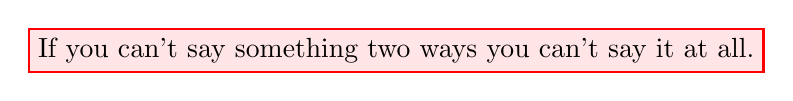
\begin{tikzpicture}
        \node[draw=red, fill=red!10, thick]
            {If you can't say something two ways you can't say it at all.};
    \end{tikzpicture}
\end{center}

This credo may seem odd to linguists, who usually take a strongly realist stance according to which the grammar formalism fully specifies the grammar, even down to notation.
For example, privative (= single-valued) and binary features are regarded as vastly different objects that make very different claims about phonology.
Yet we will see at a later point that they are but two definitions of the same computational object.
% fixme: will we see this?
That does not rule out that one of the two is a more useful way of thinking about phonology, but that is a matter of epistemology rather than ontology.

Returning from our brief methodological excursus, we now have to define bigrams, which in turn will allows us to define bigram grammars.
%
\begin{definition}[Bigrams]
    Given a string $w$ over alphabet $\Sigma$, its \emph{augmented} counterpart $\augmented{w} \is \LeftEdge \stringcat w \stringcat \RightEdge$ is obtained by adding the left and right edge markers $\LeftEdge$ and $\RightEdge$ to $w$, where $\LeftEdge$ and $\RightEdge$ are distinguished symbols not contained in $\Sigma$.
    Furthermore, 
    \(
    \Bigrams(w) \is
        \setof{
            \ngram{ab} \mid \exists u,v \in \Sigma^* \text{ s.t.\ }
                u \stringcat \ngram{ab} \stringcat v = \augmented{w}
        }
    \)
    denotes the set of \emph{bigrams} over $\augmented{w}$, i.e.\ the smallest set that contains all substrings of $\augmented{w}$ that consist of exactly $2$ symbols.
\end{definition}

\begin{definition}[Bigram Grammar]
    A \emph{bigram grammar} $G$ over alphabet $\Sigma$ is a finite set of bigrams over $\Sigma \cup \setof{\LeftEdge, \RightEdge}$.
    If $G$ is a \emph{positive bigram grammar} (denoted $\posG{G}$), then it generates the language
    \(
        L(G) \is \setof{
            w \mid \Bigrams(w) \subseteq G
        }
    \).
    If $G$ is a \emph{negative bigram grammar} (denoted $\negG{G}$), then it generates the language
    \(
        L(G) \is \setof{
            w \mid \Bigrams(w) \cap G = \emptyset
        }
    \).
\end{definition}

With all these definitions under our belt, we can finally move on to producing a new insight: positive and negative bigram grammars are equally powerful.
That is to say, if some language is generated by a positive bigram grammar, then it can also be generated by some negative bigram grammar, and the other way round.

\begin{theorem}
    The class of languages that are generated by positive bigram grammars is exactly the class of languages that are generated by negative bigram grammars.
    \label{thm:SL_PosNegEquivalence}
\end{theorem}
%
In order to show that this theorem is indeed correct, we establish two simpler propositions --- called lemmata --- which jointly imply the theorem.

\begin{lemma}
    For every positive bigram grammar there is a negative bigram grammar that generates the same language.
    \label{lem:SL_Pos2Neg}
\end{lemma}
%
\begin{proof}
    Let $\posG{G}$ be a positive bigram grammar. 
    We show that $\negG{\complementof{G}}$ defines the same language as $\posG{G}$, where $\complementof{G}$ consists of all bigrams over $\Sigma \cup \setof{\LeftEdge, \RightEdge}$ that are not contained by $G$.

    Pick some arbitrary string $w \in L(\posG{G})$. 
    By definition, every bigram of $w$ is a member of $G$, which immediately implies that no element of $\Bigrams(w)$ is contained in $\complementof{G}$.
    But if none of the bigrams of $w$ belong to $\complementof{G}$, then $\Bigrams(w) \cap \complementof{G} = \emptyset$, wherefore $w \in L(\negG{\complementof{G}})$.
    Since $w$ was arbitrary, this result holds for every string generated by $\posG{G}$, establishing $L(\posG{G}) \subseteq L(\negG{\complementof{G}})$.

    The same argument can be applied in the other direction to show $L(\posG{G}) \supseteq L(\negG{\complementof{G}})$, wherefore $L(\posG{G}) = L(\negG{\complementof{G}})$.
\end{proof}
%
This is a so-called \emph{constructive} proof: we do not just show that an equivalent negative bigram grammar exists, we also explain how this grammar can be constructed from the positive bigram grammar.
Constructive proofs are the most useful kind of proof because they provide procedures and strategies that can be implemented and run automatically.

In the case at hand, all we have to do in order to construct an equivalent negative bigram grammar is to take the set-theoretic complement of the positive bigram grammar.
After all, the set of all bigrams over $\Sigma$ is given by $\Sigma \times \Sigma$, and the positive bigram grammar $\posG(G)$ is some subset thereof (\emph{modulo} edge markers, which are treated as part of $\Sigma$ here to avoid notational clutter).
Bigrams that belong to $G$ may occur in a string, bigrams that do not must not.
So the bigrams not belonging to $G$ are the illicit bigrams, which means those are exactly the bigrams the equivalent negative bigram grammar must contain.
In one sentence: taking the complement of $G$ is like taking its negation, and the switch from a positive grammar to a negative one undoes this negation.

So now we know that the negative bigram grammars are at least as powerful as the positive bigram grammars since the latter can be translated into the former.
It only remains for us to show that the same holds in the other direction.

\begin{lemma}
    For every negative bigram grammar there is a positive bigram grammar that generates the same language.
\end{lemma}
%
\begin{proof}
    Left as an exercise to the reader.
\end{proof}
%
Figure~\ref{fig:SL_Proof} gives a pictorial representation of the implications used in these proofs.
%
\begin{figure}
\centering
\begin{tikzpicture}[
    every node/.style = {rounded corners},
    positive/.style = {draw=blue!75,fill=blue!25},
    negative/.style = {draw=red!75,fill=red!25}%
    ]
    \node[positive] (pos-member) at (0,0) {$w \in L(\posG{G})$};
    \node[positive] (subset) [below=of pos-member] {$\Bigrams(w) \subseteq G$};
    \node[negative] (disjoint) [right=5em of subset] {$\Bigrams(w) \cap \complementof{G} = \emptyset$};
    \node[negative] (neg-member) [above=of disjoint] {$w \in L(\negG{\complementof{G}})$};

    \foreach \Source/\Target in {%
        pos-member/subset,
        subset/disjoint,
        disjoint/neg-member%
        }
        \draw[<->] (\Source) to (\Target);
\end{tikzpicture}

\caption{Reasoning chain for the equivalence of positive and negative bigram grammars}
\label{fig:SL_Proof}
\end{figure}

\subsection{The How and Why of Proofs}

Proofs are a difficult art at every level of expertise.
For the beginner, the biggest challenge is often to sort out their train of thought and present it in a clear manner: where do I start, and how do I proceed from there step by step to reach the conclusion?

There are no clear-cut rules here, but it is often helpful to break up the problem into smaller ones, as we did with Thm.~\ref{thm:SL_PosNegEquivalence}.
If two sets $A$ and $B$ need to be shown to be equivalent, one can first prove $A \subseteq B$ and then $B \subseteq A$.
And a statement of the form ``$\phi$ iff $\psi$'' can be broken up into ``$\phi$ entails $\psi$'' and ``$\psi$ entails $\phi$''.
We will encounter several basic proof techniques throughout the course (proof by induction, indirect proofs), but don't worry too much about specific techniques for now.
Instead, make sure to work through the proofs we discuss multiple times until you understand how they work.
Always try to answer the following questions for yourself:

\begin{itemize}
    \item Why is the initial assumption valid?
    \item How does each conclusion follow from the previous one?
    \item Why does the final conclusion show that the theorem\slash lemma is correct?
\end{itemize}

You may wonder why we need proofs in the first place.
Linguists don't work with proofs yet they have discovered a lot of interesting things about language.
Programmers don't have much use for proofs either.
There's several answers, the simplest one being that some questions can only be addressed conclusively via proofs.
Consider the following alternative to the proof of Lem.~\ref{lem:SL_Pos2Neg}: we could have implemented the translation procedure from positive to negative grammars and then tested it on a large sample of positive bigram grammars (at least several thousand).
Eventually the program would have told us that the negative grammars generate the same string languages as their positive counterparts.
So if the conversion works correctly on every single one of thousands of positive bigram grammars, isn't that enough to posit that positive and negative bigram grammars are interchangeable?

The answer is No.
First of all, checking that two grammars generate the same language is hardly trivial if both languages are infinite (we can't just compare all their respective members).
More importantly, though, the thousands of test grammars may accidentally share a special property that is essential for the correctness of the conversion.
This is a real risk if all those test grammars were automatically generated by a script because true randomness is very hard to achieve with computers, if not impossible.
While experiments and simulations have their place --- they are a valid last resort where proofs are hard to come by --- a proof is always the preferred solution where possible.

Proofs are preferred not only because they are safe from the pitfalls of simulations, but also because they provide genuine insight.
In fact, proofs are often more important and enlightening than the theorems they establish.
Testing the correctness of the bigram conversion via automated experiments could at best show us whether the procedure is correct (if there's only finitely many cases to test), but it does not tell us \textbf{why}.
A proof is an explicit record of how certain properties entail others.
In the case at hand, it is the close connection between set-theoretic complementation and the switch from positive to negative grammars that does all the work.
Notice all the properties of bigram grammars that the proof does not depend on: that bigrams are strings, that bigrams consist of exactly two symbols, and that bigram grammars are finite. 
Yet these properties necessarily hold during any test procedure, so we would not be able to tell which one of them is a prerequisite for the correctness of the conversion.
Thanks to the proof, we know which properties matter, which in turn might come in handy in the study of other formalisms.

In a few lines, a proof can establish unassailable truths, show us why they hold, but also save us hours of work compared to running simulations.
So even though you may initially find them hard and time consuming, proofs are actually the tool of choice for the lazy scientist.


\section{Linguistic Evaluation}
The bigram grammar model improves on the list phonology model in various respects.
Variation across languages is now much more restricted because phonology is just a collection of highly local constraints (negative bigram grammars) or permissions (positive bigram grammars).
Bigram grammars also account for linguistic creativity, i.e.\ that speakers can form new words according to the rules of their own language, and that they recognize whether nonce words are well-formed.
As a consequence, they do not predict that the lexicon is finite, either.
Whether the lexicon is finite or infinite is immaterial for bigram grammars since they determine well-formedness in a compositional manner.
As long as each word is finite, its grammaticality can easily be determined via a bigram scanner.

Bigram grammars do still exhibit egalitarianism.
Since a grammar is a list of bigrams, all these bigrams should have the same status and there should be no distictions between easy and difficult processes.
For example, we have seen that the language $(\String{ab})^+$ can be generated by a bigram language.
If we identify $a$ with C and $b$ with V, we get the word template for languages that only allow CV syllables.
Clearly we could just as well have mapped $a$ to V and $b$ to C, generating a language where all words consist of VC syllables.
While many languages can have VC syllables, all languages with VC syllables also allow for CV syllables.
This implicational universal is completely unexpected if phonology is just a bigram grammar.

Isolationism is also a problem as processes still cannot apply across words.
For \emph{phone bill}, the phonological representation is presumably something like \LeftEdge\textipa{foUn}\RightEdge\LeftEdge\textipa{bIl}\RightEdge.
Since \textipa{n} and \textipa{b} are not adjacent, a negative bigram grammar with \ngram{nb} does not have the desired result.
This could be fixed with a bigger search domain, though, which also seems to be necessary for slightly less local processes like intervocalic voicing, where we want to block a voiceless sound only if it occurs between two vowels.

Overall bigram grammars are doing very well on a conceptual level and are easy to implement, but they are not expressive enough for English.
In the next chapter we will see how we can keep all their attractive properties while increasing their power to a more adequate level.

% fixme: exercises
    % - do bigram grammars use less memory than list phonology? by how much? under what circustances is this not the case?
    % - convert bigram grammar into matrix format
    % - define useless bigram
    % - show that every positive grammar has multiple equivalent negative grammars; compute their number;
    % - show that every positive grammar has exactly one equivalent negative grammar

% fixme: scanner operates in linear time

\chapter{Extending Bigram Grammars}
\label{cha:SLMath}

Bigram grammars are a step in the right direction from the initial list phonology model.
Every grammar is still just a list of items, but now we use this list to determine the well-formedness of a word in a compositional manner.
The problem of bigram grammars is that they are not powerful enough to capture certain phonological processes like intervocalic voicing --- in linguistic parlance, the size of the grammars locality domain is limited to two adjacent symbols, so bigger contexts cannot be represented correctly.
The obvious solution is to extend the size of the scanner window so that the grammar uses trigrams, 4-grams, or maybe even something bigger.
We will see today that this generalization is a natural one in the sense that it preserves the essential properties of bigram grammars while increasing their empirical coverage.

\section{Generalization to Strictly Local Grammars}

In order to generalize bigram grammars to grammars with grams of arbitrary length, we just have to change a few parameters in our original definition.
We also use this opportunity to slightly change our terminology: instead of \emph{$k$-gram grammar} and \emph{$k$-gram languages}, we will speak of \emph{strictly $k$-local grammars}.
This will make it easier later on to distinguish this formalism from a related one that also operates with $k$-grams but interprets them differently.

\begin{definition}[$k$-grams]
    A \emph{$k$-gram}, or \emph{$k$-factor}, over alphabet $\Sigma$ is an element of $(\Sigma \cup \setof{\LeftEdge, \RightEdge})^k$.
    Given a string $w$ over $\Sigma$, its \emph{$k$-augmented} counterpart $\augmented{w}_k \is \LeftEdge^{k-1} \stringcat w \stringcat \RightEdge^{k-1}$ consists of $w$ with $k-1$ left edge markers and $k-1$ right edge markers, and its set of $k$-grams is given by
    \(
        \Bigrams[k](w) \is
            \setof{
                s \in (\Sigma \cup \setof{\LeftEdge, \RightEdge})^k
                \mid
                \exists u,v \in \Sigma^* \text{ s.t. }
                u \stringcat s \stringcat v = \augmented{w}
            }
    \).
\end{definition}
%
You can see that this definition of $k$-gram is a natural extension of the concept of bigrams for if we replace $k$ by $2$ in the definition, we get exactly the original definition of bigrams.
The concept of bigram languages is generalized in the same fashion to $k$-gram languages, which jointly form the class of \emph{strictly local languages}.
%
\begin{definition}[Strictly Local Languages]
    A finite set of $k$-grams is called a \emph{strictly $k$-local grammar}.
    A positive strictly $k$-local grammar $G$ generates the language
    \(
        L(G) \is
            \setof{ w \mid \Bigrams[k](w) \subseteq G }
    \).
    A negative strictly $k$-local grammar $G$ generates the language
    \(
        L(G) \is
            \setof{ w \mid \Bigrams[k](w) \cap G = \emptyset }
    \).
    A language $L$ is \emph{strictly $k$-local} iff it is generated by some strictly $k$-local grammar.
    The class of \emph{strictly local languages} is given by
    \(
        \bigcup_{k \geq 1} \setof{ L \mid L \text{ is strictly $k$-local} }
    \).
\end{definition}
%
Intuitively, a language is strictly local iff all its well-formedness conditions are restricted to a locality domain of finitely bounded size.
\Note{%
    Notice that the definition of strictly $k$-local also allows for $k = 0$.
    Can you list all strictly $0$-local languages?
    \emph{Hint}: There's only two of them.
}

The phonological processes we have looked at so far --- word-final devoicing, nasal assimilation, and intervocalic devoicing --- are all strictly local.
The first two are strictly 2-local, the third one strictly 3-local.

It is also easy to see that constraints on syllable structure are strictly local.
Take some language that only allows for syllables of the form V, VC, CV, and CVC, but not CCV, VCC, CVCC, or CCVCC\@.
In other words, a well-formed word cannot contain more than two consecutive consonants, and these consonants cannot occur at the beginning or the end of the word, where they would necessarily be part of the same syllable.
The set of illicit substrings, then, consists of \LeftEdge CC, CCC, and CC \RightEdge.
This can be compiled out into a set of illicit sequences of phones by substituting for each C the phones that are specified for [+cons].
So this example of a restricted syllable template does note exceed the power of a negative strictly $3$-local grammar.

If desired, the negative strictly local grammar can be converted into a positive one using our standard procedure --- go back to the proof of our theorem that positive and negative bigram grammars are equivalent, you will see that it does not at all rely on the length of the $n$-grams being $2$, so the theorem can easily be generalized to all strictly local grammars.

Feel free to design strictly local grammars for other local processes in phonology, e.g.\ assimilation across word boundaries, vowel harmony, umlaut, or spirantization.
As long as these processes describe surface true generalizations --- that is to say, they do not make reference to an underlying form and can be stated purely in terms of which output forms are licit --- you should not run into any problems.
Notice that these processes must be local but can nonetheless be globally unbounded.
Vowel harmony, for instance, may apply throughout an entire word via a sequence of local vowel harmony steps.
This kind of behavior is exactly what we expect given how strictly local grammars operate: the $n$-grams only regulate the shape of local domains, but the well-formedness of the word is evaluated by moving through the word and checking each local domain.
So not only are strictly local grammars powerful enough to capture local well-formedness conditions in phonology, the way they enforce them mirrors linguists' intuitions about how local processes can produce global patterns.

The connection between strictly local grammars and local processes in phonology allows us to study the latter through the former.
Since strictly local grammars generate strictly local languages, this implies that the properties of strictly local languages can tell us something about local processes in phonology.
So now the theoretical task of proving formal properties of strictly local languages has suddenly morphed into an empirically minded investigation of phonology.

\section{Exploring Strictly Local Languages}

\subsection{A Proper Hierarchy of Strictly Local Languages}
One may expect that the power of strictly local grammars increases with the size of the locality domain.
This can indeed be shown to be the case by recourse to the strictly local languages.
If we order the strictly local languages by the size of their locality domain, we get a proper hierarchy: one level properly subsumes the next.
Denoting the class of strictly $k$-local languages by $\SL_k$, we have $\SL_k \subsetneq \SL_{k-1}$ for all $k \geq 0$.
%
\begin{lemma}
    It holds for every $k \geq 0$ that if language $L$ is strictly $k$-local, then $L$ is also $k+1$-local.
\end{lemma}
%
The proof for this lemma is slightly more complicated than anything we have seen so far, but behind the notation lies a very simple idea:
the size of the locality domain can be increased from $k$ to $k+1$ by padding the edge markers and by combining two overlapping $k$-grams into a single $k+1$-gram.
%
\begin{proof}
    If $L$ is strictly $k$-local then it is generated by some positive strictly $k$-local grammar $G$ over some alphabet $\Sigma$.
    Let $G'$ be the smallest set such that for all $k$-grams $g_1, g_2 \in G$
    %
    \begin{itemize*}
        \item if $g_1$ starts with $\LeftEdge$, then $\LeftEdge g_1 \in G'$,
        \item if $g_1$ ends with $\RightEdge$, then $g_1 \RightEdge \in G'$,
        \item if $g_1 \is a_1 a_2 \cdots a_{k}$ and $g_2 \is a_2 \cdots a_k a_{k+1}$, then $a_1 a_2 \cdots a_k a_{k+1} \in G'$.
    \end{itemize*}
    %
    Clearly $G'$ is finite and can therefore be interpreted as a positive $k+1$-local grammar.
    We show that $L = L(G')$, thus establishing that $L$ is $k+1$-local.
    
    If $w \in L(G')$, then $\Bigrams[k+1](w)$ is a subset of $G'$.
    All $k+1$-grams with multiple edge markers have a corresponding $k$-gram with one edge marker less, which is contained in $G$.
    All other $k+1$-grams are split into two $k$-grams by removing the first or the last symbol.
    Each $k$-gram is once again contained in $G$, so $\Bigrams[k](w) \subseteq G$ and hence $w \in L(G) = L$.
    Since $w$ was arbitrary we have $L(G') \subseteq L$.

    If $w \in L$, then $\Bigrams[k](w)$ is a subset of $G$.
    Assume towards a contradiction that $\Bigrams[k+1](w)$ is not a subset of $G'$.
    Then $w$ contains some $k+1$-gram $g_3$ that is not a member of $G$.
    If $g_3$ starts or ends with two edge markers, then the corresponding $k$-gram with only one of the two markers cannot have been part of $G$, contradicting our initial assumption.
    In all other cases, $g_3$ is built from two overlapping $k$-grams $g_1$ and $g_2$, at least one of which is not contained in $G$.
    But then $\Bigrams[k](w)$ is not a subset of $G$, contradicting once more our initial assumption.
    It follows, then, that $\Bigrams[k+1](w)$ is a subset of $G'$ after all, wherefore $L \subseteq L(G')$.
\end{proof}

\begin{lemma}
    For every $k$ there is some strictly $k+1$-local language that is not strictly $k$-local.
\end{lemma}
%
\begin{proof}
\Note{%
    This proof uses a finite language, but the lemma holds even if we only consider infinite languages.
    Try to generalize the proof along these lines.
}
    Consider the finite language $L$ that contains only the string $a^k$.
    It is generated by the strictly $k+1$-local grammar $\setof{\LeftEdge a^k, a^k \RightEdge}$.
    However, $\Bigrams[k](a^k) = \setof{\LeftEdge a^{k-1}, a^k, a^{k-1} \RightEdge} = \Bigrams[k](a^n)$ for every $n \geq k$, so a strictly $k$-local grammar that generates $a^k$ also generates all these $a^n$ and thus a proper superset of $L$.
\end{proof}
%
\begin{theorem}
    For all $k \geq 0$, $\SL_k \subsetneq \SL_{k+1}$.    
\end{theorem}

Now we know for sure that the size of the locality domain has a direct effect on generative capacity.
This may seem barely surprising, but it is far from trivial.
In the coming weeks we will see that for a very similar formalism, all $k \geq 2$ have exactly the same power.


\subsection{Relation to Finite Languages}

Remember that the list phonology model of Lecture~\ref{cha:ListPhonology} was restricted to lists of finite length, so it could only generate finite languages.
This restriction is empirically inadequate as it conflicts with the assumption that the list of phonological words in a given natural language is infinite and fails to handle nonce words and linguistic creativity in general.
But not only is the list phonology model restricted to finite languages, it adds insult to injury with its ability to generate all finite languages.
Every finite language is a viable natural language phonology, according to the list model, and we have already seen why this is typologically untenable.
So the class of languages that can be generated by the list phonology model is exactly the class of finite languages, which is the class that is least likely to provide an insightful or empirically adequate model of language.

The strictly local languages improve on this significantly, but only if one adopts the right perspective.
First, it is obvious that strictly local languages can be infinite, so not every strictly local language is finite.
Let us make this claim fully explicit via a proof.
We already know that every strictly $k$-local language is strictly $k+1$-local, so all we need is an example of a strictly $1$-local language.

\Note{%
Further reflection reveals that almost every $1$-local language is infinite.
In fact, there are only two $1$-local languages that are finite.
Can you define them?
\emph{Hint}: One of them is strictly $0$-local.
}
%
\begin{lemma}
    There is a strictly $1$-local language that is infinite.
\end{lemma}
%
\begin{proof}
    Let $\posG{G} \is \setof{\LeftEdge, a, \RightEdge}$.
    Then $L(\posG{G}) = \setof{\emptystring, a, \String{aa}, \String{aaa}, \ldots} = a^*$, which is infinite.
\end{proof}
%
\begin{theorem}
    For every $k \geq 1$, $\SL_k$ contains an infinite language.
\end{theorem}
%
This is a welcome result because it shows that no matter what size of locality domain we pick, we are never restricted to just finite languages.
An even more appealing property of strictly local languages is that for every level of the infinite hierarchy there are some finite languages that cannot be defined.
Consequently, strictly local grammars improve on the list phonology model in that they cannot define any arbitrary phonological systems.
%
\begin{theorem}
    For every $k \geq 1$, there is some finite language that is not contained in $\SL_k$. 
\end{theorem}
%
\begin{proof}
    Pick an infinite language that is generated by some strictly $k$-local grammar $G$ over alphabet $\Sigma$.
    Discard from $G$ all $k$-grams that start with $\LeftEdge$ or end in $\RightEdge$.
    The resulting set is a finite language $L$.
    We show that $L$ is not strictly $k$-local.

    Since $G$ generates an infinite set, it must contain (not necessarily distinct) $k$-grams $a \stringcat u$ and $u \stringcat b$, where $a,b \in \Sigma$ and $u \in \Sigma^{k-1}$.
    Note that both $a \stringcat u$ and $u \stringcat b$ belong to $L$, whereas $a \stringcat u \stringcat b$ does not.
    But $\Bigrams[k](a \stringcat u) \cup \Bigrams[k](u \stringcat b) = \Bigrams[k](a \stringcat u \stringcat b)$, and consequently every strictly $k$-local grammar that generates $a \stringcat u$ and $u \stringcat b$ also generates $a \stringcat u \stringcat b$.
    Hence $L$ is not strictly $k$-local.
\end{proof}
%
The proof above is rather sneaky.
It exploits the fact that every strictly $k$-local grammar is a finite set of strings of length $k$, which can be viewed as a finite language.
This is an interesting perspective: a strictly $k$-local grammar $G$ is a finite language $L_G$ coupled with a specific algorithm $A$ for creating a new language from $L_G$.
If we try to generate $L_G$ via a strictly $k$-local grammar, this grammar automatically uses the algorithm $A$, so for certain choices of $L_G$ the grammar generates additional strings via $A$ that do not belong to $L_G$.

Careful though: The previous theorem holds only when the size of the locality domain is fixed by some $k$.
The whole class of strictly local languages properly subsumes the class of finite languages.
%
\begin{theorem}
    Every finite language is strictly local.
\end{theorem}
%
\begin{proof}
    Suppose that $L$ is a finite language, the longest string of which has length $k - 1$, $k \geq 1$.
    We define a $k$-local grammar $G$ that consists of the $k$-grams $\LeftEdge^i \stringcat w \stringcat \RightEdge^j$, where $w \in L$, $w$ has length $l < k$, and $i + j + l = k$.
    Since every $k$-gram starts with $\LeftEdge$ or ends in $\RightEdge$, $L(G) = L$, wherefore $L$ is strictly $k$-local.
\end{proof}
%
The relation between strictly local languages and finite languages thus is more involved than one would expect.
Without restrictions on the size of the locality domain, the strictly local languages include all finite languages.
However, the class of strictly $k$-local languages and the class of finite languages are incomparable --- they have a non-empty intersection, but neither subsumes the other.
So assuming that $k$ is fixed for natural language phonology, e.g.\ as part of Universal Grammar, strictly local grammars are a good approximation of local processes in phonology.
They can handle infinity and do not incorrectly predict languages to vary freely across all dimensions.


\subsection{Substring Substitution Closure}

In several of the preceding proofs we have used the fact that a strictly local grammar sometimes ``overshoots the target''.
A finite language $L$ may not be in $\SL_k$ because a strictly $k$-local grammar that tries to generate $L$ will also end up generating other strings outside of $L$.
But a strictly $k+1$-local grammar may be able to do a point landing and generate all and only those strings that are members of $L$.
What this shows is that a strictly $k$-local grammar only has perfect precision within its locality domain of size $k$, beyond that it has to generalize.
This generalization step is what allows strictly local grammars to generate infinite languages and thus the true source of their power.

Crucially, though, strictly local grammars don't just generalize randomly, quite to the contrary: all strictly local grammars generalize in the same fashion, irrespective of the size of their locality domain.
Their generalization strategy is already implicit in the definition of strictly local languages, which categorizes strings as well-formed or ill-formed according to their set of $k$-grams.
If two strings have exactly the same set of $k$-grams, then either both are well-formed or both are ill-formed.

But it is quite hard to tell what this condition implies for the overall shape of the string languages.
Given a string language $L$, how can we tell whether $L$ is strictly local?
Fortunately strictly local languages are uniquely characterized by a property called \emph{substring substitution closure}.
%
\begin{definition}[Local Substring Substitution Closure]
    A language $L$ satisfies \emph{$k$-local substring substitution closure} iff there is some $k \geq 1$ such that if $L$ contains both $u \stringcat x \stringcat v$ and $u' \stringcat x \stringcat v'$, where $x$ has length $k - 1$, then $L$ also contains $u \stringcat x \stringcat v'$.
\end{definition}
%
\begin{theorem}
    A language is in $\SL_k$ iff it satisfies $k$-substring substitution closure.
\end{theorem}
%
Let us look at a couple of examples first before wading through the proof of the theorem.

\begin{examplebox}[A Substring Substitution Closed Language]
    We have already seen that the language $(\String{ab})^+$ is strictly $2$-local as it is generated by the grammar $\setof{\LeftEdge a, \ngram{ab}, \ngram{ba}, b \RightEdge}$.
    Now we can also verify this via substring substitution closure.
    For instance, we can line up $\String{abab}$ and $\String{abababab}$ to show that the language must also contain $\String{ababab}$.
    %
    \[
        \begin{array}{rcll}
                          & x &              & \\
            \String{ab}   & a & \String{b}   & \in L\\
            \String{abab} & a & \String{bab} & \in L\\\hline
            \String{ab}   & a & \String{bab} & \in L
        \end{array}
    \]
    %
    Notice how $x$ is a single symbol since its length must be $k-1 = 2 -1 = 1$.
    Also, we could have established the membership of $\String{ababab}$ more succinctly using just $\String{abab}$ or $\String{abababab}$.
    \[
        \begin{array}{rcll}
                        & x &              & \\
            \String{ab} & a & \String{b}   & \in L\\
                        & a & \String{bab} & \in L\\\hline
            \String{ab} & a & \String{bab} & \in L
        \end{array}
        %
        \qquad
        %
        \begin{array}{rcll}
                          & x &                & \\
            \String{ab}   & a & \String{babab} & \in L\\
            \String{abab} & a & \String{bab}   & \in L\\\hline
            \String{ab}   & a & \String{bab}   & \in L
        \end{array}
    \]
\end{examplebox}
%
Since substring substitution closure fails if even a single string is missing from the set, it is usually not a good way to of showing that a language is strictly local --- if the language in question is infinite, one cannot show via specific substitutions that it is suffix substitution closed.
However, suffix substitution closure is an excellent way of showing that a language is not strictly local by giving a single example for how one can find a missing string.
%
\begin{examplebox}[A Language that Fails Subtree Substitution Closure]
    Consider the language $(\String{aa})^+$, the variant of $(\String{ab})^+$ where all $b$s have been replaced by $a$s.
    This language is not strictly local as it fails $k$-local substring substitution closure for any choice of $k$.
    Suppose $k$ is an even number:
    %
    \[
        \begin{array}{rcll}
            & x & & \\
        a & a \cdots a & a & \in L \\
          & a \cdots a &   & \in L \\\hline
        a & a \cdots a &   & \notin L\\
        \end{array}
    \]
    %
    A similar pattern can be used if $k$ is odd.
    So no matter what the value of $k$, the language is not suffix substitution closed and thus not strictly local.
    You might find this surprising given that the only difference to $(\String{ab})^+$ is the replacement of $b$ by $a$.
    This highlights another property of strictly local languages: the alphabet plays a crucial role in what languages are definable.
\end{examplebox}
%
\begin{proof}
    To be done.
\end{proof}

\subsection{Closure Properties}

Suffix substitution closure is --- as its name implies --- a \emph{closure property}.
One says that an object $o$ is closed under an operation iff applying this operation to elements of $o$ yields only elements of $o$.
In other words, the operation never takes us outside of $o$.
The natural numbers, for instance, are closed under addition since the sum of two natural numbers is yet again a natural numbers.
But they are not closed under subtraction because, say, $2-5$ yields $-3$, which is an integer but not a natural number.
Suffix substitution closure simply means that a language is closed under the operation of substituting suffixes in a specific way.

But of course there are many other operations that can be applied to a language, and it will be interesting to see whether strictly local languages are closed under them.
In particular the basic set-theoretic operations of intersection, union, and relative complement are of interest since they tell us how we can build strictly local languages from smaller ones.

Let us look at closure under intersection first.
This one is particularly important because of the close correspondence that negative strictly local grammars establish between constraints on the one hand and languages on the other.
If every $n$-gram corresponds to a well-formedness constraints, then one would expect that one can get the intersection of two languages by simply conjoining their respective well-formedness constraints.
That is indeed the case.
%
\begin{lemma}
    The class of strictly $k$-local languages is closed under intersection, $k \geq 0$.
\end{lemma}
%
\begin{proof}
    We prove that for any two strictly local languages generated by (positive) grammars $G_1$ and $G_2$, $L(G_1) \cap L(G_2) = L(G_1 \cap G_2)$.
\Note{Give an analogous proof using negative grammars.}
    We first show $L(G_1) \cap L(G_2) \subseteq L(G_1 \cap G_2)$.
    Let $w$ be an arbitrary string belonging to both $L(G_1)$ and $L(G_2)$, i.e.\ $w \in L(G_1) \cap L(G_2)$.
    Then every $k$-gram of $w$ is contained in both $G_1$ and $G_2$, so $w \in L(G_1 \cap G_2)$.
    Since $w$ is arbitrary, we have $L(G_1) \cap L(G_2) \subseteq L(G_1 \cap G_2)$.
    The same reasoning can be applied in the other direction, yielding $L(G_1 \cap G_2) \subseteq L(G_1) \cap L(G_2)$.
    These two facts jointly imply $L(G_1) \cap L(G_2) = L(G_1 \cap G_2)$.
\end{proof}
%
% hw: spell out the second subset relation
%
Closure under intersection can also be used to prove that a language is not strictly local.
Suppose that we know that $L$ is strictly local, but we have a hard time showing that $L'$ is not strictly local.
Then we can instead try to show that $L \cap L'$ is not strictly local, as this immediately implies the non-locality of $L'$, too.

One might expect that closure under union holds too since one can simply take the union of the grammars, but this does not work as expected.
The union of two grammars $G_1$ and $G_2$ often generates a subset of the union of $L(G_1)$ and $L(G_2)$.
Do not even try to look for a smarter strategy to build a grammar for the union of two strictly local languages, there is none that works in all cases.
%
\begin{lemma}
    The class of strictly local languages is not closed under union. 
\end{lemma}
%
\begin{proof}
    We give an example of two bigram languages whose union is not a bigram language.
    The proof can easily be adapted for arbitrary values of $k$.

    Let $L_1 \is \setof{\mathit{ab}}$ and $L_2 \is \setof{\mathit{b}, \mathit{bb}, \mathit{bbb}, \ldots}$.
    Assume without loss of generality (w.l.o.g.) that all bigram grammars are positive.
    Then any bigram grammar that generates $L_1$ must contain the bigrams $\LeftEdge a$, $\mathit{ab}$, and $b \RightEdge$.
    Similarly, a bigram grammar generating $L_2$ must contain the bigrams $\LeftEdge b$, $\mathit{bb}$, and $b \RightEdge$.
    Therefore a bigram grammar that generates all strings in $L_1 \cup L_2$ must contain at least these bigrams.
    But such a grammar also generates the string $\mathit{abb}$, which is not part of $L_1 \cup L_2$.
    Hence there is no bigram grammar that generates all the strings in $L_1 \cup L_2$ and nothing else, so $L_1 \cup L_2$ is not a bigram language.
\end{proof}
%
%hw: extend proof to case where both languages are infinite
%hw: extend proof to arbitrary k

The previous two lemmata immediately imply that closure under relative complement does not hold either.
%
\begin{lemma}
    The class of strictly local languages is not closed under (relative) complement.
\end{lemma}
%
\begin{proof}
    By De Morgan's law $L_1 \cup L_2 = \complementof{\complementof{L_1} \cap \complementof{L_2}}$.
    If the class of strictly local languages were closed under both complement and intersection, it would thus be closed under union, too.
    Since closure under intersection holds while closure under union does not, closure under relative complement cannot hold, either.
\end{proof}
%
%hw: give a proof by example
You may find this result surprising because the complement of a strictly local grammar is a strictly local grammar.
But in general $\complementof{L(G)}$ differs from $L(\complementof{G})$, just like $L(G_1) \cup L(G_2)$ is not guaranteed to be $L(G_1 \cup G_2)$.
These differences illustrate why it is so important to distinguish between grammars and the languages they generate.

We finish with yet another missing closure property.
%
\begin{lemma}
    The class of strictly local languages is not closed under relabelings.
\end{lemma}
%
\begin{proof}
    We have already seen that $(ab)^+$ is strictly 2-local whereas the relabeling $(aa)^+$ is not strictly local at all.
    But the former is the image of the latter under a relabeling that replaces all $b$s by $a$s.
\end{proof}
%
This is a very important result as it ties directly into the abstractness debate in generative phonology.
Suppose that we are allowed to have all kinds of hidden structure in our phonological representation, e.g.\ a basic syllable template or feet.
Then we could assume that the language $(aa)^+$ is underlyingly equipped with a CV-template, so that we should rather think of it as $(a_C a_V)^+$.
This language is strictly local (it is a notational variant of $(ab)^+$), so $(aa)^+$ is strictly local under a mapping that removes unpronounced structure.
In later lectures we will see that this is a very dangerous route to take: hidden structure pushes strictly local languages to a level of power where all phonological processes are equally simple.
This eradicates all distinctions between processes and takes us back to the undesirable egalitarianism of the list phonology model.

\section{Implications for Phonology}
Our mathematical expedition has taught us a surprising amount about phonology.
First of all, all local phonological dependencies (including those spanning across word boundaries) can be handled by strictly local grammars, a very simple formalism with few cognitive requirements.
The model comes with a minimal memory burden as it only requires the speaker to keep track of a small number of $k$-factors.
It is also very fast: recognition via a scanner takes linear time and can be carried out in an incremental online fashion.
Lookup of $k$-factors in the grammar takes at most logarithmic time using binary search, and even fast search methods can be implemented.

But strictly local grammars also capture essential properties of phonological competence.
They are analytic in nature and thus capable of generating infinite languages, which solves the problems the list phonology model had with linguistic creativity and nonce words.
The special relation between strictly $k$-local languages and finite languages also means that certain typological pitfalls are avoided.
Not every random collection of strings is predicted to be a valid phonological system, and grammars generating an infinite language generalize in a linguistically plausible fashion by determining the well-formedness of strings as a composite function of the local domains.

We have also seen that strictly local languages lack closure properties that do not hold of natural languages either.
The union or relative complement of a natural language's phonotactics is not guaranteed to be a valid phonological system for a natural language, just like the class of strictly local languages is not closed under these operations.
The increase of power brought about by relabelings also cautions us against using hidden structures and highly abstracted alphabets, an issue that has been discussed at length in phonology and that will occupy us at various points for the rest of the course.


%hw: complete proof of positive-negative equivalence
%hw: implement translation from positive into negative bigram grammar
%hw: generalize proofs to n-grams
%hw: implement n-gram scanner

\chapter{Learning Local Dependencies}
\label{cha:LearnSL}

\begin{itemize}
    \item linguistics: explanatory adequacy directly tied to learning
    \item what is learning? what can be learned? languages, not grammars (e.g.\ we don't care if grammars have bigrams in different order)
    \item what are our parameters?
    \item learning in the limit from positive text
    \item text
    \item converge
    \item lattice learner
    \item what this paradigm ignores: cognitive load, needed sample size, frequency/indirect negative evidence, prosody, semantics, order of presentation
    \item notice how we generalize from finite set to infinite one due to how grammar is structured
\end{itemize}

\chapter{Adding Probabilities}
\label{cha:PSL}

\begin{itemize}
    \item probabilistic version: switch to different monoid (0,1,min; 0,1,*; [0,1],*)
    \item inferring probabilities
    \item smoothing techniques
\end{itemize}

\chapter{Non-Local Dependencies}
\label{cha:SP}

Our project of devising a computational model of phonological processes has made great progress.
We started out with phonology as a list of well-formed surface forms, but quickly realized that this cannot account for essential properties like linguistic creativity or that there are strong constraints on what is a possible phonological system in natural language.
So we moved to a more abstract perspective where phonology is still a list, but rather than full surface forms we list the $n$-grams that may occur in a string.
A string's well-formedness is no longer an idiosyncratic property determined by a single list lookup --- it now is contingent on the well-formedness of its parts.
We saw that this perspective equates phonological systems with strictly local languages, which allows us to explore formal properties of phonology through the study of the class of strictly local languages.
This class seems to be a good approximation of local processes: every local phonological process is captured by some strictly local language, and the class exhibits closure properties that replicate very basic typological facts.
Given a UG-specified restriction on the size of locality domains, we even get a positive learnability result under highly adversarial circumstances.
And a natural algebraic generalization in terms of monoids revealed that many of these insights do not hinge on a categorical understanding of well-formedness, they also apply in a probabilistic setting.

But linguists have discovered a lot of evidence that there is more to phonology than just local processes.
If strictly local languages do not encompass all of phonology, then the properties we have discovered so far characterize only a subpart of phonology.
The question is whether there are indeed aspects of phonology that are not strictly local, and if so, how we could revise our model in an empirically adequate fashion while maintaining the majority of the insights that we have worked so hard for.

\section{Long-Distance Dependencies in Phonology}

\subsection{Navajo Sibilant Harmony is not Strictly Local}
While many phonological processes have clearly delineated application domains of bounded size --- e.g.\ two adjacent segments, within a syllable or across a single word boundary --- some processes seem to apply across arbitrary distances.
Navajo, for instance, exhibits \emph{sibilant harmony}, where all sibilants in a word must match the anteriority of the right-most one.
For the Navajo phoneme inventory, sibilants are specified for anteriority as follows \citep[9]{Martin05}:
%
\begin{center}
    \begin{tabular}{cc}
        $[{\color{blue}+} \text{anterior}]$ & $[{\color{red}-} \text{anterior}]$\\\midrule
        \textipa{s}           & \textesh\\
        \textipa{z}           & \textyogh\\
        \textipa{ts\super h}  & \textipa{t\textesh\super h}\\
        \textipa{ts}          & \textipa{t\textesh}\\
        \textipa{ts'}         & \textipa{t\textesh'}
    \end{tabular}
\end{center}
%
Sibilant harmony applies in a variety of cases in Navajo, but it is most apparent in compounds (\citealp[10]{Martin05}; the data is presented using a mixture of Navaja orthography and IPA).
%
\begin{center}
    \begin{tabular}{ll}
        \textipa{xo{\color{red}\textesh}} & `cactus'\\
        \textipa{{\color{blue}ts}'óóz} & `slender'\\
        \textipa{xo{\color{blue}sts}'óóz} & a specific type of cactus
    \end{tabular}
    %
    \hspace{2em}
    %
    \begin{tabular}{ll}
        \textipa{{\color{red}t\textesh}aa} & `ear'\\
        \textipa{néé{\color{blue}z}} & `long'\\
        \textipa{{\color{blue}ts}aanéé{\color{blue}z}} & `mule'
    \end{tabular}
\end{center}
%
Since there is no upper bound on how many words a compound may consist of, and since the evidence suggests sibilant harmony can hold across an unbounded number of words within a compound, we are dealing with a truly unbounded process.
We can express this as a formal theorem.
%
\begin{theorem}
    Sibilant harmony is not strictly local.
\end{theorem}
%
\begin{proof}
    This could be proved by exhibiting a productive pattern of Navajo compounding such that two sibilants with distinct anteriority values can be arbitrarily far apart from each other.
    Instead, we first convert sibilant harmony into a more abstract string language, and we then show that this string language is not strictly $k$-local for any choice of $k$.

    Let $l$ be a relabeling that replaces anterior sibilants by $a$, non-anterior sibilants by $b$, and all other segments by $c$.
    Then sibilant harmony is satisfied in all strings over alphabet $\setof{a,b,c}$, and only those, that do not contain both $a$ and $b$.
    Let $L$ be the set of all such strings.
    Then $L$ contains strings $s_{a,i} \is \String{a c^i a}$ and $s_{b,i} \is \String{b c^i b}$.
    Suppose $L$ is strictly $k$-local.
    By $k$-local suffix substitution closure, $s_{a,k} \in L$ and $s_{b,k} \in L$ jointly imply $\String{c^k a c^k b c^k} \in L$.
    But this string violates sibilant harmony and thus cannot be a member of $L$, showing that $L$ is not strictly $k$-local.
    Since $k$ was arbitrary, $L$ is not strictly local.
\end{proof}

Note that the proof starts out with a relabeling.
At an earlier point we proved that strictly local languages are not closed under relabelings, so strictly speaking this proof cannot establish that sibilant harmony is not strictly local.
Rather, it shows that sibilant harmony is not strictly local if one assumes that segments that aren't sibilants contribute no useful information for determining well-formedness with respect to sibilant harmony.

From a linguistic perspective, this means that any tricks that might allow us to decompose the long-distance dependency into a local one are banned unless they have a visible effect on the surface form.
For example, we cannot use anything like ``invisible spreading'' where the right sibilant has some feature that invisibly spreads to the adjacent segment to the right, and from there to the next one, and so one, until it reaches another sibilant and changes the value of anteriority feature.
This is important to keep in mind: our claims about the complexity of various phonological processes are stated with the shared understanding that no hidden structure or distinctions can be invoked.
Such hidden structures might exist, of course, but positing them blurs important boundaries and ties our claims to a very specific theoretical interpretation of the data --- one that might easily be false.
Before we try to unify distinct phenomena by recourse to more elaborate structures, we should try to discern to which degree these phenomena are actually distinct.

\subsection{Strictly Piecewise Languages}

Now that we have encountered a process that is not strictly local, we have to start looking for a model that is sufficiently powerful but not too different from strictly local languages and grammars.
At good starting point is to take another gander at the proof above --- determining which property of strictly local languages was used to establish their inadequacy will give us an idea what needs to be changed.
Adopting for a moment the perspective of a strictly $k$-local scanner, we quickly see the problem.
In order to regulate the dependency between $a$ and $b$, both have to be within the scanner's search window, but that is impossible whenever the distance between the two exceeds the size of the search window.
But what if our search window wasn't in one solid piece, but could be broken up into smaller parts that move around independently?
That is to say, what if a strictly $k$-local scanner didn't have $1$ window of size $k$, but $k$ windows of size $1$?

Suppose that we have such a scanner, with $2$ windows of size $1$.
Then a string satisfies sibilant harmony iff it can never be the case that one of the windows is on an anterior sibilant and the other window on a non-anterior sibilant.

\subsection{Properties of Strictly Piecewise Languages}

Since strictly piecewise languages are the result of coupling the format of strictly local grammars with a different method for determining string well-formedness --- precedence instead of adjacency --- all the proofs that rely only on the grammar format carry over without modifications.
This implies immediately that we can freely convert between positive and negative SP grammars, and that $\SP_k$ is learnable in the limit from positive text for every $k$.
Other properties require only a little bit of extra work.
The proof for closure under intersection is easily adopted, as is the proof for non-closure under union (and thus relative complement).
The argument that all finite languages are strictly local also establishes that they are strictly piecewise, which furthermore entails that $\SP$ is not learnable in the limit from positive text.

The strictly piecewise languages thus retain all essential properties of the strictly local languages, which isn't too surprising seeing how they are both generated by $n$-gram formalisms.
These properties line up very well with what we know about phonology --- they do not give a full characterization of phonology, but what they do claim seems to be along the right track.
It is very tempting to surmise that natural language phonology is somewhere in the union of $\SL_j$ and $\SP_k$ for some UG-specified values of $j$ and $k$.
In other words, phonology can be factored into a finite number of local and non-local processes that each correspond to some strictly local or strictly piecewise language (closure under intersection ensures that these can all be combined into two systems of local and non-local processes, respectively).

\Note{
    \centering
    \includegraphics[width=2.75cm]{./img/pic/heinz_crop.png}

    \noindent
    \textbf{Jeffrey Heinz}
}
Jeffrey Heinz has advocated this position in a series of papers \citep{Heinz10,HeinzIdsardi11}, but only for segmental phonology.
Suprasegmental phenomena, in particular stress, are exempt from this claim.
And this is a good thing since some suprasegmental phenomena fall outside the purview of $\SL$ and $\SP$.

\section{Suprasegmental Phonology}

\subsection{Unbounded Stress}
One phenomenon we haven't considered so far is stress assignment.
Every language comes with a fixed set of rules that determine which syllable in a word gets primary stress and is thus prosodically most prominent. 
Sometimes primary stress assignment can even resolve lexical ambiguities, such as in English with the noun \emph{$'$export} and verb \emph{ex$'$port}.

Most languages use rather simple stress assignment rules, such as \emph{stress the first syllable} (which we will call \textbf{[0]} following Python's indexation system) or \emph{stress the antepenultimate} (abbreviated \textbf{[-3]}).
These simple systems are strictly local.
Consider \textbf{[0]}, and assume that our alphabet consists of $s$ and $u$ for stressed and unstressed syllables, respectively.
Then the set of (non-empty) strings that are well-formed with respect to \textbf{[0]} is exactly the language of the positive strictly $2$-local grammar $\setof{\ngram{\LeftEdge s}, \ngram{su}, \ngram{uu}, \ngram{u\RightEdge}}$.
For \textbf{[-3]}, we need a strictly $4$-local grammar such that $\ngram{suu\RightEdge}$ is the only $4$-gram containing $\RightEdge$ and no other $4$-gram starts with $s$.
%
\Note{%
    The high values for $k$ might actually indicate that phonological structures have two levels, one for segmental phonology and one for suprasemental phonology, with local processes on each level limited to some low $k$.
    This would explain why stress patterns require a high $k$ over segmental structures while all other local segmental processes operate within considerably smaller domains.
}
Since there is an upper bound on the length of syllables (probably around 9, since some languages have very complex syllables like CCCVVCCCC) these grammars can be generalized to our standard string models where each segment represents a sound rather than a syllable.
The values for $k$ will be high ($18$ and $36$, respectively), but there is a finite upper bound that renders these stress patterns strictly local.

But there are some stress patterns where the position of primary stress is more flexible and varies with the structure of the word.
Kwakwala, for instance, exhibits what \citet{Hayes95} calls a \emph{Leftmost Heavy Otherwise Right} (LHOR) pattern:
%
\begin{description}
    \item[LHOR] Primary stress falls on the leftmost heavy syllable in a word, and if there are no heavy syllables, on the final syllable.
\end{description}
%
Suppose that this pattern were strictly 2-local, given an alphabet of H and L for unstressed heavy and non-heavy syllables, respectively, and \'{H} and \'{L} for their stressed counterparts.
Then the corresponding positive $\SL_2$ grammar must contain at least the bigrams \'{L}\RightEdge\ (stress falls on the final syllable) and \'{H}L (stress falls on a heavy syllable).
But this grammar will also accept strings where stress falls on a heavy syllable that is not leftmost.
Since there is no principled upper bound on the distance between two heavy syllables, or the distance between a heavy syllable and the left edge of a word, we cannot fix this issue by moving to an $\SL_k$ grammar.
So we need to bring in aspects of $\SP$.
To this end, we combine the positive $\SL_2$ grammar with a negative $\SP_2$ grammar that consists only of the bigram H\'{H}.
Now we correctly capture the fact that the only valid targets for primary stress are the final syllable and the leftmost heavy syllable.

But this is not enough to enforce LHOR\@:
The $\SL_2$ grammar and the $\SP_2$ grammar accept strings where primary stress falls on both the leftmost heavy syllable and the final syllable.
In order to rule out this case, we add the bigrams \'{H}\'{H} and \'{H}\'{L} to the $\SP_2$ grammar, so that a string can only contain one primary stress.
Unfortunately this is still insufficient, because both grammars will accept strings containing no stressed syllable at all.
Try as we might, there is no way around this due to how these grammars calculate well-formedness: if $w$ is well-formed, then so is every string $w'$ with $\Bigrams[k](w') \subseteq \Bigrams[k](w)$.
For any string $w$ with a stressed syllable, the grammars also accept every string $w'$ that can be built from those $k$-grams of $w$ that mention no stressed syllable.
So $\SL$ allows us to tie stress to absolute positions in the string, and $\SP$ can identify relative positions as well as put an upper bound on how many stressed syllables a word may contain, but neither can enforce a lower bound in the general case.
Our grammars can \emph{allow} specific configurations to occur in a string, but they cannot \emph{force} them to occur if a local alternative is available.

\subsection{Culminativity and Threshold Testability}

The problematic property of stress patterns like LHOR is that every string has to contain exactly one primary stress, which \citet{Heinz14} calls \emph{culminativity}.
The union of $\SL$ and $\SP$ can ensure the presence of at most one primary stress but fails to enforce the ``at least one'' half of the requirement.
What we need, then, is a way to enforce lower bounds like this.

The most obvious solution is to pair a grammar $G$ with a function $\ThreshFunc$ that associates with each $k$-gram $g$ a threshold $\ThreshFunc(g)$.
This threshold establishes the minimum number of times that a $k$-gram must appear in a string.
%
\begin{definition}[Strict Threshold Testability]
    A \emph{strictly $k$-local\slash piecewise $m$-threshold testable grammar} is a pair $\tuple{G,\ThreshFunc}$ such that
    %
    \begin{itemize}
        \item $G$ is a positive strictly $k$-local\slash $k$-piecewise grammar, and
        \item $\ThreshFunc: G \rightarrow [0,m]$ is a total function assigning to each $k$-gram of $G$ a \emph{threshold} less than $m$.
    \end{itemize}
    %
    Given a string $w$, $\StringOcc{g}{w}$ denotes the number of occurrences of $k$-gram $g$ in $w$.
    The language generated by $G$ is $L(G) \is \setof{ w \mid \StringOcc{g}{w} \geq \ThreshFunc(g) }$.
    % The class of all strictly $k$-local\slash piecewise $m$-threshold testable languages is denoted by $\SLTT{k}{m}/\SPTT{k}{m}$.
    % A language $L$ is \emph{strictly threshold testable} (\STT) iff it is $\SLTT{k}{m}$ or $\SPTT{k}{m}$ for some fixed $k$ and $m$.
    A language $L$ is \emph{strictly threshold testable} (\STT) iff it is strictly $k$-local\slash piecewise $m$-threshold testable for some fixed $k$ and $m$.
    % If $m = 1$, we just call $L$ \emph{strictly testable}.
\end{definition}
%
Assuming an abstract alphabet where we distinguish only stressed and unstressed syllables, culminativity is expressed by the strictly $1$-local $1$-threshold testable grammar $G \is \setof{\tuple{\String{s},1},\tuple{\String{u},0}}$ (this is a more compact representation that defines $G$ and $\ThreshFunc$ at the same time).
Since the 1-gram $\String{s}$ has threshold $1$, every string must contain at least one primary stress, whereas it need not contain any unstressed syllables.
The negative strictly piecewise grammar from the previous section blocks all strings with more than $1$ strings, so the intersection of the languages generated by these two grammars contains only strings with exactly one primary stress.
So culminativity can be factored into a strictly piecewise grammar and a $1$-local $1$-threshold testable grammar --- in other words, it requires merely the smallest conceivable extension of the strictly local and strictly piecewise languages.

A problem arises, though, if we want both grammars to use the same alphabet and thus distinguish between stressed and unstressed heavy and non-heavy syllables.
In this case $G$ needs to be expanded into
\(
    G \is \setof{
        \tuple{\String{\text{\'H}},1},
        \tuple{\String{\text{\'L}},1},
        \tuple{\String{\text{H}},0},
        \tuple{\String{\text{L}},0}
    }
\).
But this means that every string must contain at least one stressed heavy syllable and at least one stressed non-heavy syllable.
This is clearly not what we want, and there isn't a single string that can satisfy this requirement and at the same time be generated by the strictly piecewise grammar.
Culminativity thus is strictly threshold testable, but only over an impoverished alphabet.
This is, in a certain sense, the inverse of previous cases where certain languages turned out to be strictly local only if one uses a refined alphabet that provides hidden information.
Nonetheless it shows once more that the choice of alphabet is an important factor for determining the complexity of a process or constraint.

Another debatable assumption is that the application domain of phonology is a single word.
This is clearly not the case for segmental processes, which can apply across word boundaries.
The default assumption is that suprasegmental processes thus should not be limited to a single word, either.
But that means that the input may include, among other things, a sequence of two mono-syllabic words, both of which must carry primary stress.The string could thus contain, say, \LeftEdge \'H\RightEdge\LeftEdge \'L\RightEdge.
This is blocked by the $\SP_2$ grammar's bigram \'H\'L\@ but can be remedied by moving to a positive $\SP_4$ grammar whose $4$-grams may contain two stressed syllabes only if they are separated by \RightEdge\LeftEdge.
More problematically, the ill-formed \LeftEdge \'H\RightEdge\LeftEdge L\RightEdge is predicted to be grammatical --- neither the $\SP_4$ grammar nor the strictly threshold testable grammar block it.

Our approach to culminativity thus hinges on specific assumptions about the alphabet and the domain within which suprasegmental phonological processes apply.
Following our standard methodology of conservatively adding new mechanisms and testing their limits we could carefully map out a space of increasingly more powerful formalisms and see how culminativity fits into these classes depending on our assumptions.
This would reveal that culminativity over the expanded alphabet requires the power of so-called \emph{locally testable grammars} (a generalization of strictly local $1$-testable grammars), while extending the domain beyond words means moving to the much more powerful class of \emph{star-free grammars}.
Instead of exploring all these subtly different formalisms, we will turn our attention to a more principled investigation of the role of hidden structure as it is commonly entertained by phonologists.
In particular, how much power can we obtain by distinguishing identical phones via a hidden alphabet?

% hw: write monoid functions for extracting all n-sequences
% hw: adopt proofs

\chapter{\texorpdfstring{Hidden Alphabets \emph{or} The Horrors of Abstractness}{Hidden Alphabets or The Horrors of Abstractness}}
\label{cha:REG}

\section{Adding a Hidden Alphabet}

\subsection{Refined Strictly Local Grammars}

\begin{definition}[Run]
    Let $\Sigma$ and $Q$ be overt and \emph{hidden} alphabets, respectively.
    Each $q \in Q$ is called a \emph{state}.
    Given a string $w$ over $\Sigma$, a \emph{$(\Sigma,Q)$-run} over $w$ is a total function mapping each node $n$ of $w$ to some $q \in Q$.
    We also say that \emph{$q$ is assigned to $n$}, and we represent the set of all $(\Sigma,Q)$-runs over $w$ by $Q^w$.
    We may omit mention of $\Sigma$ and $Q$ if they are clear from the context.
    Overloading our terminology, we also use run to refer to the image of $w$ under a given run, or the string of pairs $p_1 \cdots p_n$, where each $p_i$ consists of the $i$-th node of $w$ and its image under some fixed $Q$-run.
\end{definition}
%
\begin{examplebox}[Runs Over a Short String]
    Suppose that $Q \is {p,q,r}$ and that $w \is \String{abbca}$.
    Then the set of $Q$-runs over $w$ includes, among others, $qpprq$, $pqrpq$, or even $ppppp$, but not $qppqs$ (because $s \notin Q$), $qpp$ (too few symbols), or $pqrpqr$ (too many symbols).
    If we view runs as strings of pairs, then the three runs and non-runs look as below:
    %
    \begin{center}
        \begin{tabular}{ccccc}
            $q$ & $p$ & $p$ & $r$ & $q$\\
            $a$ & $b$ & $b$ & $c$ & $a$
        \end{tabular}
        %
        \hspace{1em}
        %
        \begin{tabular}{ccccc}
            $p$ & $q$ & $r$ & $p$ & $q$\\
            $a$ & $b$ & $b$ & $c$ & $a$
        \end{tabular}
        %
        \hspace{1em}
        %
        \begin{tabular}{cccccc}
            $p$ & $p$ & $p$ & $p$ & $p$ & \phantom{$r$}\\
            $a$ & $b$ & $b$ & $c$ & $a$ &
        \end{tabular}
        
        \vspace{1em}

        \begin{tabular}{ccccc}
            $q$ & $p$ & $p$ & $q$ & $s$\\
            $a$ & $b$ & $b$ & $c$ & $a$
        \end{tabular}
        %
        \hspace{1em}
        %
        \begin{tabular}{ccccc}
            $q$ & $p$ & $p$ &     &\\
            $a$ & $b$ & $b$ & $c$ & $a$
        \end{tabular}
        %
        \hspace{1em}
        %
        \begin{tabular}{cccccc}
            $p$ & $p$ & $p$ & $p$ & $p$ & $r$\\
            $a$ & $b$ & $b$ & $c$ & $a$ &
        \end{tabular}
    \end{center}
\end{examplebox}

\begin{definition}[Refined Grammar]
    A refined strictly $k$-local grammar $G$ is a finite set of $k$-grams over alphabet $\Sigma \times Q$.
    Such a grammar generates the language $L(G) \is \setof{ w \mid \exists r \in Q^w, \Bigrams[k](r) \subseteq G}$.
    A language is refined strictly $k$-local iff it is generated by a refined strictly $k$-local grammar.
    The class of all refined strictly $k$-local languages is denoted $\SL_k^R$.
\end{definition}
%
\begin{examplebox}[A Refined Grammar for Even Counting]
    Recall that the language $(\String{aa})^+$, which contains all non-empty strings over $a$ whose length is even, is neither strictly local nor strictly piecewise.
    However, it can be generated by a refined strictly $2$-local grammar with only a handful of bigrams.
    %
    \begin{center}
        \begin{tabular}{cccc}
            \kState{eo}{\LeftEdge a} &
            \kState{oe}{a a} &
            \kState{eo}{a a} &
            \kState{ee}{a \RightEdge}
        \end{tabular}
    \end{center}
    %
    This grammar generates $\String{aaaa}$, for instance, because there is a run such that each bigram of that run is licensed by the grammar.
    In contrast, the slightly longer $\String{aaaaa}$ is not generated because every run contains at least one bigram that is not licensed by the grammar.
    We indicate this by not assigning a state to the node for which an irreconcilable conflict arises.
    %
    \begin{center}
        \begin{tabular}{cccccc}
            e & o & e & o & e & e\\
            \LeftEdge & a & a & a & a & \RightEdge
        \end{tabular}
        %
        \hspace{2em}
        %
        \begin{tabular}{ccccccc}
            e & o & e & o & e & o & \\
            \LeftEdge & a & a & a & a & a & \RightEdge
        \end{tabular}
    \end{center}

\end{examplebox}

\subsection{Generative Capacity}

Due to how refined strictly local grammars are defined, they trivially subsume the strictly local grammars as a special case where the hidden alphabet $Q$ contains only one state.
The fact that a refined strictly $2$-local grammar can generate $(\String{aa}^+)$ shows that the inclusion is proper --- refined strictly local grammars are strictly more powerful than strictly local grammars without a hidden alphabet of states.
But this result can be even strengthened: ever strictly local language is refined strictly $2$-local.
%
\begin{lemma}
    $\SL \subsetneq \SL_2^R$
\end{lemma}
%
To see this, just keep in mind that in order to determine the well-formedness of a string with respect to a strictly $k$-local grammar, it suffices to memorize all the $k$-grams in the string and see if all of them are licensed by the grammar.
This was exactly the way our first scanner implementation operated.
In a refined strictly local grammar, we can use the states to keep track of all the $k$-grams, and the only states that can be assigned to the right edge marker $\RightEdge$ are those that represent a subset of the strictly $k$-local grammar.

\begin{proof}
    We already have $\SL_2^R \not\subseteq \SL$ thanks to the example of $(\String{aa})^+$, so it suffices to show $\SL \subseteq \SL_2^R$.
    Let $L \in SL_k$ be a language over alphabet $\Sigma$, and $G$ a positive strictly $k$-local grammar such that $L(G) = L$.
    The grammar $G_2^R$ is the largest subset of $(\Sigma \times Q)^2$ such that
    %
    \begin{itemize}
        \item $Q$ consists of pairs $\tuple{g,S}$, where $g$ is a $k$-gram and $S$ a set of $k$-grams over $\Sigma$,
        \item $\kState{pq}{ab} \in G_2^R$ only if, for $p \is \tuple{g_p,S_p}$ and $q \is \tuple{g_q,S_q}$
            \begin{itemize}
                \item if $a = \LeftEdge$, then $p \is \tuple{\LeftEdge^k, \setof{\LeftEdge^{k-1} \cdot b}}$,
                \item $g_q \is u \cdot b$, where $u \in \Sigma^{k-1}$ and $g_p \is x \cdot u$,
                \item $S_q \is S_p \cup \setof{g_q}$,
                \item $S_q \subseteq G$.
            \end{itemize}
    \end{itemize}
    
    Since $S_q$ must be a subset of $G$, it follows immediately that $L(G^R_2) \subseteq L(G)$. 
    In the other direction, suppose that some $w \in L(G)$ is not contained in $L(G^R_2)$.
    Then there is no $r \in Q^w$ for which $\Bigrams[k](r) \subseteq G^R_2$.
    However, $G^R_2$ is a maximal subset and thus contains every $\kState{pq}{ab}$ unless one of the conditions above is violated.
    But since $w \in L(G)$, $\Bigrams[k](w) \subseteq G$, so $g_p$, $g_q$ and $S_q$ are well-defined, and $S_q \subseteq G$.
\end{proof}

The strategy above can be modified to keep track of subsequences instead of substrings, which entails that every strictly piecewise language is refined strictly $2$-local.
And because $(\String{aa}^+$ is not strictly piecewise but refined strictly $2$-local, we get yet another proper subsumption relation.
%
\begin{lemma}
    $\SP \subsetneq \SL_2^R$
\end{lemma}
%
At this point it shouldn't come as a surprise that even the strict threshold testable languages are refined strictly $2$-local.
%
\begin{lemma}
    $\STT \subsetneq \SL_2^R$
\end{lemma}
%
\begin{proof}
    Left as an exercise to the reader.
\end{proof}

As you can see, the addition of a hidden alphabet has made our formalism much more powerful, to the extent where we can't even make any distinctions between local and non-local dependencies: they all belong to $\SL_2^R$.
And as we will see next, things are even worse insofar as locality plays no role at all in refined strictly local grammars.


\section{The Loss of Locality}

\subsection{Reduction to 2-Locality}

\begin{theorem}
    If a language is generated by a refined strictly $k$-local grammar with hidden alphabet $Q$ ($k \geq 2$) then it is generated by a refined strictly $2$-local grammar with hidden alphabet $Q'$.
    \label{thm:REG_SL2}
\end{theorem}
%
The proof for this theorem is fairly cumbersome to read, but the intuition of the construction is very simple: since a refined strictly $k$-local grammar has only a finite number of $k$-grams, we can emulate the computations of the whole grammar in our hidden alphabet.
%
\begin{examplebox}[Emulating a Grammar via a Hidden Alphabet]
    Let $L$ be the language of all strings over $\setof{a,b}$ such that consecutive substrings of $b$s must have even length and may only occur after at least three $a$s. 
    \label{ex:REG_HiddenTranslation}
    This language includes strings like $\String{aaa}$, $\String{aaabb}$, and $\String{aaabbbba}$, but not $\String{bbaaa}$ or $\String{aaab}$.
    This can be easily handled by a refined strictly $4$-local grammar where the hidden alphabet keeps track of the length requirement while the presence of three $a$s is enforced directly via the $4$-grams.
    The initial $4$-grams are very simple, since no $b$ can occur at the start of a string:
    %
    \[
        \begin{array}{cccc}
            \kState{eeee}{\LeftEdge \LeftEdge \LeftEdge a} &
            \kState{eeee}{\LeftEdge \LeftEdge a a} &
            \kState{eeee}{\LeftEdge a a a} &
        \end{array}
    \]
    %
    The final $4$-grams already have to take quite a bit of variation into account:
    %
    \[
        \begin{array}{cccc}
            \\[12pt]
            \kState{eeee}{a \RightEdge \RightEdge \RightEdge} &
            \kState{eeee}{a a \RightEdge \RightEdge} &
            \kState{eeee}{a a a\RightEdge} &
            \kState{eoee}{a b b\RightEdge}
            \\[12pt]
            \kState{eeee}{b \RightEdge \RightEdge \RightEdge} &
            \kState{eeee}{b a \RightEdge \RightEdge} &
            \kState{eeee}{b a a\RightEdge} &
            \\[12pt]
            \kState{oeee}{b b \RightEdge \RightEdge} &
            \kState{oeee}{b b a \RightEdge} &
            \\[12pt]
            \kState{eoee}{b b b \RightEdge}
        \end{array}
    \]
    %
    The non-initial, non-final $4$-grams are also much fewer than one might expect thanks to the restricted distribution of $b$s:
    %
    \[
        \begin{array}{ccccc}
            \kState{eeee}{aaaa} &
            \kState{eeeo}{aaab} &
            \kState{eeoe}{aabb} &
            \kState{eoee}{abba} &
            \kState{eoeo}{abbb}
            \\[12pt]
            \kState{eoeo}{bbbb} &
            \kState{oeoe}{bbbb} &
            \kState{eoee}{bbba} &
            \kState{oeee}{bbaa} &
            \kState{eeee}{baaa}
        \end{array}
    \]
    %
    Let's quickly verify that this grammar generates the string $\String{aaabb}$ but not $\String{aaabbabb}$ or $\String{aaabbaaab}$.
    %
    \[
        \begin{array}{ccccccccccc}
                e & e & e & e & e & e & o & e & e & e & e\\
                \LeftEdge & \LeftEdge & \LeftEdge & a & a & a & b & b & \RightEdge & \RightEdge & \RightEdge
        \end{array}
    \]
    \[ 
        \begin{array}{ccccccccccccccc}
                e & e & e & e & e & e & o & e & e & e & & & & &\\
                \LeftEdge & \LeftEdge & \LeftEdge & a & a & a & b & b & a & a & b & b &\RightEdge & \RightEdge & \RightEdge
        \end{array}
    \]
    \[ 
        \begin{array}{ccccccccccccccc}
                e & e & e & e & e & e & o & e & e & e & e & o & & &\\
                \LeftEdge & \LeftEdge & \LeftEdge & a & a & a & b & b & a & a & a & b &\RightEdge & \RightEdge & \RightEdge
        \end{array}
    \]
    
    We are now going to convert this grammar into a refined strictly $2$-local one.
    The operation is very simple to carry out: every $4$-gram is first split into two $3$-grams, one of which includes the first three positions, the other one the last three positions.
    We then use these two $3$-grams as the hidden symbols for the $2$-gram that consists of the last two positions of the $4$-gram.
    For example, $\dfrac{eoee}{abba}$ is turned into the bigram below.
    %
    \[
        \dfrac{
            \dfrac{eoe}{abb}
            \dfrac{oee}{bba}
            }
            {
            b\quad a
            }
    \]
    %
    The whole grammar consists of the following bigrams (the translation also produces a few refined bigrams for $\String{\RightEdge \RightEdge}$, but those are never useful in a strictly $2$-local grammar and can safely be discarded):
    \[
        \begin{array}{ccccc}
            \kState{
                \kState{eee}{\LeftEdge \LeftEdge \LeftEdge}
                \kState{eee}{\LeftEdge \LeftEdge a}
                }
                {
                \LeftEdge \quad a
                }
            &
            \kState{
                \kState{eee}{\LeftEdge \LeftEdge a}
                \kState{eee}{\LeftEdge a a}
                }
                {
                a \quad a
                }
            &
            \kState{
                \kState{eee}{\LeftEdge a a}
                \kState{eee}{a a a}
                }
                {
                a \quad a
                }
            \\[12pt]
            \kState{
                \kState{eee}{a a a}
                \kState{eee}{a a \RightEdge}
                }
                {
                a \quad \RightEdge
                }
            &
            \kState{
                \kState{eoe}{a b b}
                \kState{oee}{b b \RightEdge}
                }
                {
                b \quad \RightEdge
                }
            &
            \kState{
                \kState{eee}{b a a}
                \kState{eee}{a a \RightEdge}
                }
                {
                a \quad \RightEdge
                }
            &
            \kState{
                \kState{oee}{b b a}
                \kState{eee}{b a \RightEdge}
                }
                {
                a \quad \RightEdge
                }
            &
            \kState{
                \kState{eoe}{b b b}
                \kState{oee}{b b \RightEdge}
                }
                {
                b \quad \RightEdge
                }
            \\[12pt]
            \kState{
                \kState{eee}{a a a}
                \kState{eee}{a a a}
                }
                {
                a \quad a
                }
            &
            \kState{
                \kState{eee}{a a a}
                \kState{eeo}{a a b}
                }
                {
                a \quad b
                }
            &
            \kState{
                \kState{eeo}{a a b}
                \kState{eoe}{a b b}
                }
                {
                b \quad b
                }
            &
            \kState{
                \kState{eoe}{a b b}
                \kState{oee}{b b a}
                }
                {
                b \quad a
                }
            &
            \kState{
                \kState{eoe}{a b b}
                \kState{oeo}{b b b}
                }
                {
                b \quad b
                }
            \\[12pt]
            \kState{
                \kState{eoe}{b b b}
                \kState{oeo}{b b b}
                }
                {
                b \quad b
                }
            &
            \kState{
                \kState{oeo}{b b b}
                \kState{eoe}{b b b}
                }
                {
                b \quad b
                }
            &
            \kState{
                \kState{eoe}{b b b}
                \kState{oee}{b b a}
                }
                {
                b \quad a
                }
            &
            \kState{
                \kState{oee}{b b a}
                \kState{eee}{b a a}
                }
                {
                a \quad a
                }
            &
            \kState{
                \kState{eee}{b a a}
                \kState{eee}{a a a}
                }
                {
                a \quad a
                }
        \end{array}
    \]
    %
    When we use this grammar to determine the well-formedness of the previous three example strings, we once again see that only the first one has a run and is thus generated by the grammar.
    %
    \[
        \begin{array}{ccccccc}
                \ComplexState{eee}{\LeftEdge \LeftEdge \LeftEdge} &
                \ComplexState{eee}{\LeftEdge \LeftEdge a} &
                \ComplexState{eee}{\LeftEdge a a} &
                \ComplexState{eee}{a a a} &
                \ComplexState{eeo}{a a b} &
                \ComplexState{eoe}{a b b} &
                \ComplexState{oee}{b b \RightEdge}
                \\
                \LeftEdge & a & a & a & b & b & \RightEdge 
        \end{array}
    \]
    \[ 
        \begin{array}{ccccccccccc}
                \ComplexState{eee}{\LeftEdge \LeftEdge \LeftEdge} &
                \ComplexState{eee}{\LeftEdge \LeftEdge a} &
                \ComplexState{eee}{\LeftEdge a a} &
                \ComplexState{eee}{a a a} &
                \ComplexState{eeo}{a a b} &
                \ComplexState{eoe}{a b b} &
                \ComplexState{oee}{b b a} &
                \ComplexState{eee}{b a a} &
                \\
                \LeftEdge & a & a & a & b & b & a & a & b & b &\RightEdge
        \end{array}
    \]
    \[ 
        \begin{array}{ccccccccccc}
                \ComplexState{eee}{\LeftEdge \LeftEdge \LeftEdge} &
                \ComplexState{eee}{\LeftEdge \LeftEdge a} &
                \ComplexState{eee}{\LeftEdge a a} &
                \ComplexState{eee}{a a a} &
                \ComplexState{eeo}{a a b} &
                \ComplexState{eoe}{a b b} &
                \ComplexState{oee}{b b a} &
                \ComplexState{eee}{b a a} &
                \ComplexState{eee}{a a a} &
                \ComplexState{eeo}{a a b} &
                \\
                \LeftEdge & a & a & a & b & b & a & a & a & b &\RightEdge
        \end{array}
    \]
\end{examplebox}
%
As this example shows, we never need a search window bigger than $2$ because the hidden alphabet can keep track of all the extra information a bigger window would provide.
Turning this intuition into a proof is fairly straight-forward, but requires a loot of bookkeeping via indices.
%
\begin{proof}
    We show that every strictly $k$-local grammar $G_k$ with refined alphabet $\tuple{\Sigma_k,Q_k}$ can be converted into a strictly $2$-local grammar $G_2$ with refined alphabet $\tuple{\Sigma_k,(\Sigma_k \times Q_k)^{k-1}}$ such that $L(G_k) = L(G_2)$.
    Let $G_2$ be the smallest set of bigrams such that if $g \is \dfrac{q_1 \cdots q_k}{\sigma_1 \cdots \sigma_k}$ is a $k$-gram of $G_k$, then $G_2$ contains $g' \is \dfrac{\phi \rho}{\sigma_{k-1} \sigma_k}$, where $\phi \is \dfrac{q_1 \cdots q_{k-1}}{\sigma_1 \cdots \sigma_{k-1}}$ and $\rho \is \dfrac{q_2 \cdots q_k}{\sigma_2 \cdots \sigma_k} \in Q_k^{k-1}$.
    We give an inductive proof that $L(G_2) = L(G_k)$.

    Suppose $w \in L(G_k)$, and that $g_k \is \dfrac{q_1 \cdots q_k}{\sigma_1 \cdots \sigma_k}$ is the refined $k$-gram spanning from the $m$-th to the $(m+k-1)$-th symbol of the $k$-augmented counterpart $\augmented{w}_k$ of $w$.

    For the base case assume $m = 1$.
    Then the first $k-1$ symbols of $g_k$ are left edge markers: $\sigma_i = \LeftEdge$, $1 \leq i < k$, while the $2$-augmented counterpart $\augmented{w}_2$ lacks the first $k-2$ symbols of $\augmented{w}_k$.
    Given the construction above, $G_2$ contains the refined bigram
    \[
        g_2 \is 
        \dfrac{
            \dfrac{
                q_1 \cdots q_{k-1}}
                {\sigma_1 \cdots \sigma_{k-1}}
            \cdot
            \dfrac{
                q_2 \cdots q_k}
                {\sigma_2 \cdots \sigma_k}
            }
            {\LeftEdge\qquad \sigma_k},
    \]
    which can be assigned to the first two positions of $\augmented{w}_2$.
    In the other direction, if $g_2$ is assigned to the first $2$ positions of $\augmented{w}_2$, then $g_k$ can be assigned to the first $k$ positions of $\augmented{w}_k$.
    Since $g_2 \in G_2$ iff $g_k \in G_k$, the first $2$ positions of $\augmented{w}_2$ are well-formed wrt $G_2$ iff the first $k$ positions of $\augmented{w}_k$ are well-formed with respect to $G_k$.

    For arbitrary $m$, suppose that $g_k$ spans from the $m$-th to the $n$-th position of $\augmented{w}_k$, where $n = m + k - 1$.
    By our induction hypothesis, some bigram spans the positions in $\augmented{w}_2$ that correspond to $n - 2$ and $n - 1$ of $\augmented{w}_k$--- namely $n - (k - 2) - 2 = m - 1$ and $n - (k - 2) - 1 = m$, respectively.
    Moreover, the second component of this bigram is
    %
    \[
        \dfrac{
            \dfrac{
                q_1 \cdots q_{k-1}}
                {\sigma_1 \cdots \sigma_{k-1}}
            }
            {\sigma_{k-1}}
            .
    \]
    By our construction, then, there is a $g_2 \in G_2$ that spans from $m$ to $m+1$ and has the shape
    \[
        \dfrac{
            \dfrac{
                q_1 \cdots q_{k-1}}
                {\sigma_1 \cdots \sigma_{k-1}}
            \cdot
            \dfrac{
                q_2 \cdots q_k}
                {\sigma_2 \cdots \sigma_k}
            }
            {\sigma_{k-1}\qquad \sigma_k}
    \]
    iff $g_k \in G_k$.
\end{proof}

Theorem~\ref{thm:REG_SL2} shows that every refined strictly local language is refined strictly $2$-local.
Rather than the infinite hierarchies of increasing complexity that we saw with the strictly local and strictly piecewise languages, this class is flat, at least with respect to whether a language can be generated by a refined strictly $2$-local language.
To emphasize this flatness, we don't just drop the locality parameter --- which might be mistaken as refering to a more powerful class that is the union of all refined strictly $k$-local languages --- but coin a completely new term.
%
\begin{definition}[Regular Languages]
    A language is \emph{regular} iff it is generated by a refined strictly $2$-local grammar.
\end{definition}
%
Regular languages are one of the most important classes of string languages in computer science and have been defined in numerous equivalent ways.
We do not have time to look at all of them, but most of them are covered in every decent textbook on formal language theory such as \citet{Sipser05}, \citet{Kozen97}, or \citet{HopcroftUllman79} (listed in increasing order of difficulty).

At least one of these equivalent definitions of regular languages can be inferred rather easily from example~\ref{ex:REG_HiddenTranslation}, though.
In this example, we saw that parts of a $k$-gram can be crammed into the hidden alphabet of a bigram.
But in principle we could do the same thing to the bigram and copy the overt symbols into the hidden alphabet, too.
In this case, we can infer the state of a node purely from the label of that node and the state of the preceding node; the label of the preceding state is no longer needed.
Consequently, every bigram $\kState{p q}{b a}$ can be represented by a simple graph.
%
\begin{center}
    \begin{tikzpicture}
    \node[state] (in) {p};
    \node[state] (out) [right=of in] {q};

    \path[->] (in) edge node [above] {a} (out);
\end{tikzpicture}

\end{center}
%
We can think of this graph as a machine or \emph{automaton} that switches from state $p$ to $q$ if it reads in an $a$.
The whole grammar is an automaton that combines the mini-automata of all the bigrams.
For the language in example~\ref{ex:REG_HiddenTranslation}, the automaton is actually much easier to understand than the refined grammar we constructed.
%
\begin{center}
    \input{./img/tikz/REG_3aEvenbAutomaton.tikz}
\end{center}
%
The graph uses start to indicate which state(s) may be assigned to the first node, whereas only circled states may be assigned to the final node.
The runs for the three test strings from the previous example now look slightly different, but they still lead to the same conclusions.
%
\[
    \begin{array}{ccccc}
            0 & 1 & 2 & o & e\\
            a & a & a & b & b 
    \end{array}
\]
\[ 
    \begin{array}{ccccccccc}
            0 & 1 & 2 & o & e & 0 & 1 & &\\
            a & a & a & b & b & a & a & b & b 
    \end{array}
\]
\[ 
    \begin{array}{ccccccccc}
            0 & 1 & 2 & o & e & 0 & 1 & 2 & o\\
            a & a & a & b & b & a & a & a & b 
    \end{array}
\]

\begin{definition}[Finite-State Automaton]
    A \emph{finite state automaton} (FSA) is a quintuple $A \is \tuple{\Sigma, Q, I, F, \Delta}$, where
    %
    \begin{itemize}
        \item $\Sigma$ is an alphabet,
        \item $Q$ is a finite set of states,
        \item $I \subseteq Q$ is the set of \emph{initial} states,
        \item $F \subseteq Q$ is the set of \emph{final} states,
        \item $\Delta \subseteq Q \times \Sigma \times Q$ is a finite set of transition rules.
    \end{itemize}
    %
    The FSA is \emph{deterministic} iff $I$ is a singleton set and $\Delta$ contains no two $\tuple{p,a,q}$ and $\tuple{p,a,r}$ with $q \neq r$.
    Otherwise it is non-deterministic.
\end{definition}

determinization via powerset construction

\section{Properties of Regular Languages}

cylindrification

boolean closure

relabeling closure

closure under reversal

Myhill-Nerode characterization

closure under finite-state transductions


\bibliographystyle{../../linquiry3}
\bibliography{../../universal,../../graf}
\end{document}
